% ============================================================================
% main.tex  --  Minimum wages and workers by education level in Peru
% Compiles with pdflatex + bibtex (author-year via natbib/apalike), or tectonic.
%   pdflatex main ; bibtex main ; pdflatex main ; pdflatex main
% ============================================================================
\documentclass[12pt]{article}

\usepackage[utf8]{inputenc}
\usepackage[T1]{fontenc}
\usepackage{lmodern}
\usepackage[english]{babel}
\usepackage{amsmath,amssymb,amsthm}
\usepackage{graphicx}
\usepackage{booktabs}
\usepackage{threeparttable}
\usepackage{caption}
\usepackage{subcaption}
\usepackage{float}
\usepackage[margin=1in]{geometry}
\usepackage{setspace}
\usepackage[authoryear,round]{natbib}
\bibliographystyle{apalike}
\usepackage[hidelinks]{hyperref}
\usepackage{xcolor}
\usepackage{siunitx}
\usepackage{enumitem}

\captionsetup{font=small,labelfont=bf}
\setlength{\parskip}{2pt}
\graphicspath{{../figures/}{figures/}}

\newcommand{\Low}{\mathrm{Low}}
\newcommand{\Post}{\mathrm{Post}}

\title{\textbf{Minimum Wages and Workers by Education Level:\\
Evidence from Peru's 2022 Reform}\thanks{This paper uses the public-use quarterly
employment modules of the Encuesta Nacional de Hogares (ENAHO) of the Instituto
Nacional de Estad\'istica e Inform\'atica (INEI). All estimates use survey weights;
the replication package is available in the accompanying repository. All errors are
the author's own.}}

\author{Eric Torres Ram\'irez\\
  \small Ph.D.\ candidate, Pontificia Universidad Cat\'olica del Per\'u\\
  \small \texttt{etorresram@gmail.com}}
\date{This version: \today}

\begin{document}
\maketitle

\begin{abstract}
\noindent
Whether a minimum wage helps the workers it targets depends on how many of them it
reaches. I study Peru's May 2022 increase in the national minimum wage, from 930 to
1,025 soles. Because Peru sets a single national minimum wage, the reform reaches every
worker at the same time, and identification comes from differences in exposure by
education rather than from staggered timing: low-education workers cluster at the wage
floor and are bound by it, while high-education workers earn well above it and provide a
lower-exposure comparison group. Using sixteen quarters of the Peruvian national
household survey (ENAHO, 2021--2024) and a difference-in-differences event study, I find
that the reform did not raise the real hourly wages of low-education workers relative to
high-education workers. This wage null is precise, holds across the wage distribution, and
reappears around the January 2025 increase. Around 2022 I also find a shift from formal
employment toward self-employment, concentrated among youth and women, but this margin is
less robust and does not replicate in 2025. In a labor market with pervasive informality
and weak enforcement, the minimum wage reallocates low-skilled workers across employment
arrangements more than it raises their pay, a pattern that qualifies the ``lighthouse''
view of the Peruvian minimum wage found for earlier reforms.

\medskip
\noindent\textbf{Keywords:} minimum wage; informality; education; difference-in-differences; Peru.\\
\noindent\textbf{JEL codes:} J23, J31, J38, J46, O17.
\end{abstract}

\medskip
\noindent\textbf{Highlights}
\begin{itemize}[nosep,leftmargin=1.4em]
\item Effects of Peru's 2022 minimum wage identified from exposure gaps by education.
\item Real wages of low-education workers did not rise relative to high-education workers.
\item The precise wage null reappears around the January 2025 minimum wage increase.
\item Formal employment fell and self-employment rose in 2022, but not robustly.
\item With high informality, the wage floor reallocates workers more than it lifts pay.
\end{itemize}

\newpage
\onehalfspacing

\section{Introduction}\label{sec:intro}

The employment effects of the minimum wage remain among the most debated questions
in labor economics, and the debate is sharper still in developing countries, where a
large share of the workforce operates outside the reach of labor regulation. In such
settings a statutory wage floor can raise pay for covered workers, push some of them
into the uncovered informal sector, or serve as a coordinating reference for wages
that formal firms would have set in any case. Which of these forces dominates is an
empirical question whose answer depends on how binding the floor is, how strictly it
is enforced, and how easily workers and firms move between the formal and informal
margins. This paper studies these questions for Peru, a country that combines a high
statutory minimum wage relative to median pay with one of the highest rates of labor
informality in Latin America.

We exploit the increase in Peru's national minimum wage (the \emph{Remuneraci\'on
M\'inima Vital}, or RMV) from 930 to 1,025 soles, enacted by Supreme Decree
003-2022-TR and effective on 1 May 2022. This 10.2 percent nominal increase was the
first change to the RMV in four years, and it occurred as the labor market was
emerging from the pandemic. A central institutional fact shapes the analysis: Peru
sets a single national minimum wage, with no regional or sectoral variation in the
general regime. There is therefore no cross-sectional variation in the level of the
policy and no staggered adoption to exploit. As \citet{jimenez_2023} notes for the
2016 reform, credible identification must instead come from differential
\emph{exposure} to a policy that changes for everyone at the same time.

Our source of differential exposure is education. In the pre-reform quarters the
median monthly wage of a dependent employee in Peru was almost exactly 930 soles,
the old minimum, so the typical low-education worker sat right at the wage floor. A
10 percent increase in that floor is highly binding for such workers. High-education
workers, by contrast, have a median wage well above the minimum and are far less likely to
be bound by its level, although some remain exposed through informal or own-account work.
This gap in exposure, rather than a claim of zero exposure for the comparison group,
motivates a difference-in-differences design that
contrasts low-education workers (those with at most complete secondary schooling,
who make up roughly two thirds of the working-age population) with high-education
workers (those with any tertiary schooling). The design follows a long tradition of
measuring minimum wage effects from variation in the ``bite'' of the policy across
groups or regions \citep{card_1992, lee_1999, machin_manning_rahman_2003}, adapted
here to a setting with a single national reform and rich, quarterly household data.

We use the public-use quarterly employment modules of the Encuesta Nacional de
Hogares (ENAHO) from the first quarter of 2021 through the fourth quarter of 2024,
sixteen quarters that bracket the reform with five pre-reform and eleven post-reform
periods. The panel structure of the data at the quarterly frequency lets us estimate
a dynamic event study, test for differential pre-trends by skill, and trace the path
of effects for more than two years after the reform. We examine a broad set of
outcomes: real hourly wages and monthly earnings, the probability of employment and
of labor force participation, the incidence of formal versus informal employment,
hours of work, and the composition of employment between wage work and
self-employment. Throughout we use survey weights and cluster inference by
department, and we complement conventional cluster-robust standard errors with the
small-sample correction of \citet{pustejovsky_tipton_2018} and with randomization
inference, because the treatment is assigned at a coarse level.

Three findings emerge. First, the reform did not raise the real wages of
low-education workers relative to high-education workers. The estimated effect on the
log real hourly wage is a precisely estimated null, and the event study shows no
break at the reform and flat pre-trends. This is our most robust result. Second, the
reform is associated with a decline in the probability that a low-education worker
holds formal salaried employment and with an offsetting rise in self-employment, a
pattern consistent with reallocation from the formal to the informal margin rather
than with the compression of the formal wage distribution documented for earlier
Peruvian reforms. Third, the employment rate of low-education workers falls modestly
relative to that of high-education workers, though this margin is the least robust
and is sensitive to the treatment of the pandemic recovery quarter of early 2021.
For the wage and formality results, pre-trends are statistically flat; for
employment and self-employment they are not, and we address this directly using the
sensitivity analysis of \citet{rambachan_roth_2023} and a battery of specification
and placebo checks. We further replicate the entire design on the subsequent reform
of January 2025, which raised the RMV to 1,130 soles in a cleaner, post-pandemic
window, and obtain a consistent picture.

Our contribution is threefold, and we are careful not to overstate it. First, we
provide the first evaluation of the 2022 Peruvian minimum wage reform and, to our
knowledge, the first study of any Peruvian reform using the post-pandemic quarterly
ENAHO. The existing micro evidence for Peru stops at the 2016 reform
\citep{jimenez_2023} or the reforms of the early 2000s \citep{jaramillo_lopez_2006,
cespedes_2005}. Second, we make heterogeneity by education the central object of
analysis at the worker level. Prior work cuts heterogeneity by income range or age,
or constructs a department-level ``dose'' of exposure; none contrasts low- and
high-education workers directly as treatment and comparison groups in an event study
of the Peruvian minimum wage. Third, we place the informal margin at the center of
the analysis and show that the adjustment to the reform runs through the composition
of employment rather than through pay. We do not claim novelty for the underlying
identification idea, which is the standard exposure or bite design, nor for the
econometric toolkit, which is by now well established. The value added is the
combination of a new reform, a new and policy-relevant period, an education-based
worker-level design, and a careful treatment of the informal margin and of the
threats to identification that such a design entails.

The remainder of the paper is organized as follows. Section~\ref{sec:institutional}
describes the Peruvian minimum wage and the reform. Section~\ref{sec:literature}
reviews the related literature. Section~\ref{sec:data} presents the data and the
construction of the key variables. Section~\ref{sec:strategy} sets out the empirical
strategy and the identifying assumptions. Section~\ref{sec:results} reports the main
results, Section~\ref{sec:robustness} the robustness and inference checks, and
Section~\ref{sec:heterogeneity} the heterogeneity and distributional analysis.
Section~\ref{sec:discussion} discusses mechanisms, external validity, and
limitations, and Section~\ref{sec:conclusion} concludes.

\section{Institutional background}\label{sec:institutional}

\subsection{The Peruvian minimum wage}

Peru sets a single national minimum wage, the \emph{Remuneración Mínima Vital}
(RMV), which applies to workers in the private-sector labor regime. Unlike federal
systems such as the United States or Brazil, and unlike countries with occupational
or regional wage floors, Peru has no sub-national or industry-specific statutory
minimum in the general regime. A small number of activities carry fixed multiples of
the RMV (for example the mining premium and the agricultural daily wage), but these
are pegged mechanically to the national value and move with it.\footnote{These pegged
regimes, such as the agrarian and mining regimes and the small-enterprise (MYPE) regime,
move one-for-one with the RMV and so introduce no cross-sectional variation in its level.} The consequence for
research design is decisive: because the level of the RMV is common to the whole
country, there is no cross-sectional variation in the policy and no staggered timing
of adoption. Any credible research design must therefore exploit differences in how
exposed workers are to a change that reaches everyone simultaneously.

In principle the RMV is to be adjusted periodically by the tripartite National Labor
Council in line with inflation and productivity. In practice the Council has never
set the RMV, and the level is fixed at the discretion of the executive through a
Supreme Decree. Adjustments are consequently infrequent and irregular in both timing
and magnitude, and Peru is among the most volatile minimum wage setters in the
region \citep{jimenez_2023, cespedes_2005}. The RMV had stood at 930 soles since
April 2018.\footnote{Fixed by Supreme Decree 004-2018-TR. The two preceding increases raised
the RMV from 750 to 850 soles in May 2016 and from 850 to 930 soles in April 2018, so the
2022 reform followed an unusually long freeze.}

Two features make the RMV unusually binding by international standards. First, its
ratio to the median wage is high. In my pre-reform sample the national median
monthly wage of a dependent employee is almost exactly 930 soles, so the old minimum
already sat at the median of the covered wage distribution and the Kaitz index, the
ratio of the minimum to the median wage, is close to one nationally and well above
one in the poorer departments. Second, compliance is far from universal. Consistent
with earlier work \citep{jaramillo_lopez_2006, cespedes_2005}, a large share of
workers earn below the statutory floor, especially in rural areas, in small firms,
and in the informal sector, while compliance inside registered formal firms is high.
Enforcement capacity is limited.\footnote{Labor inspection is the responsibility of the
National Superintendency of Labor Inspection (SUNAFIL), whose inspection staff is thin
outside Lima. Earlier work estimates overall non-compliance with the RMV at roughly 30 to
40 percent, concentrated in rural areas, small firms, and the informal sector
\citep{jaramillo_lopez_2006, cespedes_2005}.} These features imply that a nominal increase in the
RMV can bind mechanically for formal workers near the floor while leaving much of the
informal sector formally uncovered, so that the policy's real reach depends on the
degree of informality and on the ease of movement across the formal and informal
margins.

\subsection{The 2022 reform}

The reform I study was enacted by Supreme Decree 003-2022-TR, signed on 2 April 2022
and published on 3 April, and took effect on 1 May 2022. It raised the RMV from 930
to 1,025 soles, an increase of 95 soles or 10.2 percent, the first change in four
years. Figure~\ref{fig:mw} plots the nominal and real value of the RMV over
2021--2025. Two points are worth noting. The nominal increase of 10.2 percent was
partly offset by inflation, which ran at roughly 8 percent over 2022, so the increase
in the real value of the floor was more modest and eroded over the following two
years. This tempers the expected size of any wage response and is relevant when
comparing my estimates with those from lower-inflation episodes. The reform also
occurred during the post-pandemic recovery, a period of unusual labor market
turbulence that I address explicitly in the empirical analysis.

A second reform, enacted by Supreme Decree 006-2024-TR and effective on 1 January
2025, raised the RMV further to 1,130 soles. This change falls just outside my main
study window, but the ENAHO quarters for 2025 are available and I use this second
reform as an out-of-sample replication of the design in Section~\ref{sec:robustness}.
The two reforms are of very similar magnitude, 10.2 percent each, which makes the
2025 episode a natural validation exercise in a calmer, post-pandemic environment.

\begin{figure}[H]
\centering
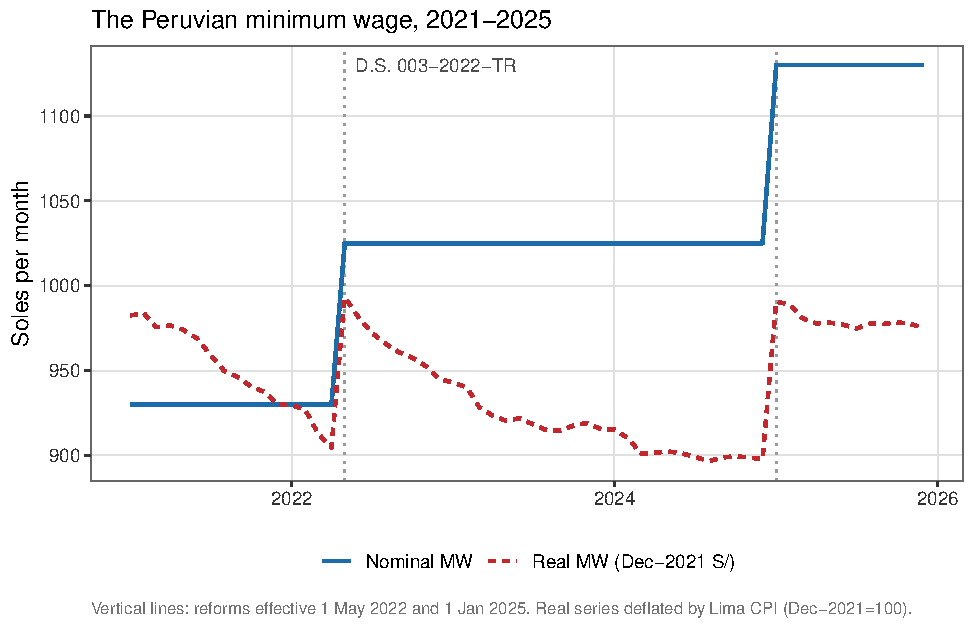
\includegraphics[width=0.82\textwidth]{fig1_minimum_wage.pdf}
\caption{The nominal and real Peruvian minimum wage, 2021--2025. The real series is
deflated by the Lima consumer price index (December 2021 = 100). Vertical dotted
lines mark the reforms effective 1 May 2022 (Supreme Decree 003-2022-TR) and 1
January 2025 (Supreme Decree 006-2024-TR).}
\label{fig:mw}
\end{figure}

\section{Related literature}\label{sec:literature}

My paper connects three strands of research: the theory and evidence on minimum
wage employment effects, the evidence for developing countries with large informal
sectors, and the specific literature on Peru.

\paragraph{Theory and the canonical evidence.} The competitive model predicts that a
binding wage floor reduces employment among low-productivity workers, with an effect
whose size depends on labor demand elasticities and on the fraction of workers bound
by the floor \citep{brown_1999}. Models with employer wage-setting power deliver
different predictions: under monopsony a moderate minimum wage can raise employment,
and it typically compresses the lower tail of the wage distribution
\citep{manning_2003}. The empirical literature has moved from a presumption of sizable
disemployment toward a consensus of small effects on the margin studied. The case
study of \citet{card_krueger_1994} and the broader synthesis in \citet{card_krueger_1995}
found little evidence of job loss from the New Jersey reform, and the border-discontinuity
design of \citet{dube_lester_reich_2010} and the bunching approach of
\citet{cengiz_2019} likewise find that recent United States increases raised wages at
the bottom with limited employment effects; \citet{manning_2021} reads the accumulated
evidence as an ``elusive'' employment effect, while \citet{neumark_wascher_2007} offer
the skeptical reading. \citet{harasztosi_lindner_2019} show that a large Hungarian
increase was absorbed mostly through prices rather than employment. Closest to my
mechanism, \citet{dustmann_2022} show that the German minimum wage operated through
\emph{reallocation}---moving workers across establishments---rather than through
employment losses, and \citet{engbom_moser_2022} document how a rising Brazilian
minimum compressed the formal wage distribution; \citet{derenoncourt_montialoux_2021}
trace distributional consequences of coverage extensions in the United States.
A recurring theme, which I build on directly, is that effects should be measured
where the minimum ``bites.'' \citet{card_1992} uses regional variation in the
fraction of workers affected, \citet{clemens_wither_2019} follow workers whose wages
sat below a rising federal floor, \citet{lee_1999} uses the gap between the minimum and
the median wage, and \citet{machin_manning_rahman_2003} exploit a low-wage sector in
which the introduction of the United Kingdom minimum was especially binding. My
education-based design is an application of the same logic to a single national reform.

\paragraph{Developing countries and informality.} In economies with large informal
sectors the minimum wage interacts with the boundary between covered and uncovered
work, and two opposing forces appear repeatedly. A ``lighthouse'' effect can raise
wages even in the informal sector, where the minimum serves as a norm or reference
\citep{lemos_2009, bosch_manacorda_2010, maloney_nunez_2004}, while a reallocation
effect can push workers out of formal employment and into informal or self-employed
arrangements \citep{ham_2018_honduras}; \citet{ulyssea_2018} provides the modern
equilibrium framework in which regulation shifts firms and workers across the
formality boundary. The Latin American evidence spans this range. Early work on
Mexico and Colombia found disemployment where the floor was high relative to wages
\citep{bell_1997}, and \citet{gindling_terrell_2007} show for Costa Rica that legal
floors move wages only in the covered sector. Studies of Brazil find wage compression
with small employment effects and evidence of spillovers into the informal sector
\citep{lemos_2009, lemos_2004}; \citet{jales_2018} estimates, with a density
approach, that the Brazilian minimum moves a substantial share of workers into
informality. Work on Ecuador finds positive wage effects concentrated among
low-income workers \citep{wong_2019_ecuador}, and \citet{arango_2022_colombia}
collect the recent Colombian evidence. The Honduran case is the clearest
counterexample to the lighthouse view: \citet{ham_2018_honduras} documents that a
high minimum wage reduced covered employment and shifted workers toward informality,
with no reduction in poverty. For Uruguay, \citet{katzkowicz_2021_uruguay} use a
density-discontinuity approach in the domestic-work sector to show that effects
concentrate among the least skilled. The common methodological thread is the use of
exposure or bite measures, either geographic Kaitz indices or fraction-affected
shares, and a careful accounting of the informal margin, both of which I adopt.

\paragraph{Peru.} The domestic literature is thin and, until recently, dated; the
margin I emphasize has, however, begun to attract attention, with
\citet{corcuera_2024} studying the response of informal self-employment to Peruvian
minimum wage increases in earlier data. Early
studies of the reforms of the early 2000s find small and often statistically weak
effects. \citet{jaramillo_lopez_2006} analyze the 2003 increase using short quarterly
panels for metropolitan Lima and conclude that the reform was largely innocuous, with
negative employment-retention effects concentrated near the floor and evidence of
displacement from the formal to the informal sector. \citet{cespedes_2005} estimates a
weakly significant employment elasticity of about $-0.13$ and shows that the RMV
Granger-causes formal wages, an early statement of the lighthouse view for Peru. The
most credible modern study is \citet{jimenez_2023}, who evaluates the 2016 reform using
a difference-in-differences design with a department-level treatment dose, defined as
the pre-reform share of formal workers earning between the old and new minimum. That
study finds no disemployment, a rise in formality of 2.5 to 2.8 percentage
points, and wage gains of 4.1 to 5.4 percent, and it interprets the pattern
through employer market power, of the kind \citet{amodio_deroux_2021} document
directly in Colombian manufacturing plants. My paper differs from this precedent in three
respects that I make explicit. I study a later reform and the post-pandemic period;
I define exposure at the worker level through education rather than at the department
level; and I find a different pattern of adjustment, with no wage gain and a decline
rather than an increase in formality. I return to the reconciliation of these
findings in Section~\ref{sec:discussion}. As \citet{jimenez_2023} emphasizes, the
binding constraint for any Peruvian design is the absence of sub-national variation in
the nominal minimum, which forces the researcher to manufacture differential exposure;
my contribution is to do so through the education dimension and to trace the
consequences for the formal and informal margins.

\paragraph{Econometrics of difference-in-differences.} Methodologically I rely on the
modern difference-in-differences literature. Because my reform occurs at a single
date, the recent concerns about negative weighting and forbidden comparisons under
staggered adoption \citep{goodmanbacon_2021, dechaisemartin_2020, sun_abraham_2021,
callaway_santanna_2021} do not bind: with a common treatment date the two-way
fixed-effects estimator and its event-study analog are unbiased for a convex average
of group-time effects \citep{roth_2023_trending, baker_larcker_wang_2022}. I
nonetheless use the doubly robust estimator of \citet{santanna_zhao_2020} as a
building block, and I take the threat to identification, namely differential trends
by skill, seriously through the sensitivity analysis of \citet{rambachan_roth_2023}.
For inference with few clusters I follow \citet{bertrand_2004},
\citet{cameron_2008_bootstrap}, and \citet{pustejovsky_tipton_2018}; selection into
the wage sample is bounded with the trimming approach of \citet{lee_2009}.
Distributional effects are estimated with the unconditional quantile method of
\citet{firpo_fortin_lemieux_2009}.

\section{Data and measurement}\label{sec:data}

\subsection{The ENAHO quarterly employment modules}

I use the public-use quarterly files of the Encuesta Nacional de Hogares (ENAHO),
the national household survey conducted by Peru's Instituto Nacional de Estad\'istica
e Inform\'atica (INEI). ENAHO is a nationally representative, stratified,
multi-stage survey with continuous fieldwork; the quarterly employment and income
module (module 500) records detailed labor market information for each household
member of working age. I pool the sixteen quarters from the first quarter of 2021
through the fourth quarter of 2024, which yields about 347,000 person-quarter records
of working-age individuals, and I add the four quarters of 2025 for the out-of-sample
validation exercise. All statistics use the module's sampling weights; the treatment of
standard errors is discussed in Section~\ref{sec:strategy}.

I restrict the sample to individuals of working age, defined as ages 14 to 65, and
I drop observations with missing education. My main wage analysis is further
restricted to dependent wage employees, for whom the minimum wage is the relevant
statutory floor, while the employment, participation, formality, and self-employment
outcomes are defined over the working-age population or over the employed, as
appropriate.

\subsection{Education and the definition of skill groups}

The treatment and comparison groups are defined by educational attainment, recorded
in ENAHO variable \texttt{p301a}, the highest level of schooling completed. I
validated the coding of this variable against the weighted distribution of attainment
in the data; it corresponds to the standard INEI classification, ranging from no
schooling through postgraduate study. I define \emph{low-skilled} workers as those
with at most complete secondary schooling (no education, initial, primary, or
secondary), and \emph{high-skilled} workers as those with any tertiary schooling
(non-university higher, university, or postgraduate). I exclude the small residual
category of special education, which is not ordered on the skill dimension, and
observations with missing education.

This partition has three attractive features. First, it is a bright line in the
Peruvian labor market: completion of tertiary schooling is the main credential that
separates workers who compete for jobs paying near the minimum wage from those who do
not. Second, it splits the working-age population into groups of comparable size,
roughly two thirds low-skilled and one third high-skilled, which gives adequate
statistical power on both sides. Third, and most important for identification, the two
groups differ sharply in their exposure to the minimum wage. As
Table~\ref{tab:desc} shows, in the pre-reform period the median monthly wage of a
low-skilled dependent employee is close to the statutory floor, whereas the median
high-skilled employee earns well above it. The classification follows a long line of
work that treats education as a primary determinant of where the minimum wage bites
\citep{lemos_2009, katzkowicz_2021_uruguay}.

\subsection{Outcome variables}

The outcomes fall into three groups. On \emph{pay}, the real hourly wage is monthly labor
income in the main occupation divided by monthly hours, deflated by the Lima consumer price
index to December 2021 soles and winsorized at the first and last half-percentiles; I build
monthly labor income following the ENAHO convention of \citet{jimenez_2023}, and real monthly
earnings is the same numerator without the hours adjustment. On \emph{quantities}, employment
and labor force participation are indicators defined over the working-age population, and
weekly hours is hours worked in the main occupation. On \emph{composition}, formal employment,
self-employment, and an indicator for being paid below the statutory minimum are defined among
the employed; the last is a direct measure of the bite of and compliance with the policy.

A measurement issue arises for informality. INEI's official informal-employment
indicator, \texttt{ocupinf}, is present in the 2021 through 2023 files but is not
released in the 2024 and 2025 files. Because my study window extends through 2024, I
reconstruct a consistent informality indicator from underlying primitives that are
available in every year: pension affiliation, the possession of a formal labor
contract, the registration status of the productive unit, and the category of
employment. I validate the reconstruction against the official \texttt{ocupinf} in
2021 through 2023, where both are available, and obtain agreement of about 88 percent
at the worker level, with an implied informality rate within one percentage point of
the official figure. I use the official indicator wherever it exists and the
reconstruction only for 2024 and 2025, and I report a robustness check that restricts
the formality analysis to the years covered by the official measure. Full details of
the construction are in Appendix~\ref{app:data}.

\subsection{Descriptive statistics}

Table~\ref{tab:desc} reports weighted means of the main variables by skill group in
the pre-reform period. The two groups differ in the expected ways. Low-skilled
workers are older on average, more likely to be male and rural, and have far lower
wages. The employment rate is similar across groups, but the composition of
employment differs starkly: low-skilled workers are much more likely to be informal
and self-employed, and far more likely to earn below the statutory minimum. Roughly
seven in ten employed low-skilled workers earn below the new minimum in the pre-reform
period, against fewer than four in ten high-skilled workers, which is the exposure gap on
which my design rests. The high informality of the low-skilled group,
around 85 percent against about 49 percent for the high-skilled, is central to
interpreting the results: for most low-skilled workers the statutory floor is not
directly enforced, so the margin along which the labor market can adjust is the
allocation of workers across formal and informal arrangements rather than the level of
pay within formal jobs.

\begin{table}[H]\centering
\caption{Descriptive statistics by skill group, pre-reform period}\label{tab:desc}
\begin{threeparttable}
\begin{tabular}{lccc}
\toprule
 & Low-skilled & High-skilled & Difference \\
 & ($\le$ sec. complete) & ($\ge$ higher) & \\
\midrule
Age & 35.92 & 34.65 & 1.27 \\
Female & 0.50 & 0.50 & 0.00 \\
Urban & 0.76 & 0.93 & -0.17 \\
Married & 0.53 & 0.41 & 0.12 \\
Years of education & 8.57 & 14.47 & -5.90 \\
Labour force participation & 0.73 & 0.80 & -0.07 \\
Employed & 0.69 & 0.73 & -0.04 \\
Wage employee (incl. domestic) & 0.29 & 0.48 & -0.19 \\
Self-employed & 0.39 & 0.24 & 0.15 \\
Formal (if employed) & 0.13 & 0.47 & -0.34 \\
Informal (if employed) & 0.87 & 0.53 & 0.34 \\
Weekly hours (if employed) & 39.74 & 41.44 & -1.70 \\
Real hourly wage (S/) & 5.74 & 9.08 & -3.34 \\
Real monthly earnings (S/) & 904.30 & 1,755.12 & -850.82 \\
Below MW (wage earners) & 0.43 & 0.19 & 0.24 \\
\midrule
Observations & 65,954 & 27,278 & \\
\bottomrule
\end{tabular}
\begin{tablenotes}\footnotesize
\item Notes: Weighted means using ENAHO survey weights, working-age individuals (14--65) in the pre-reform quarters (2021Q1--2022Q1). Low-skilled: education at most complete secondary (\texttt{p301a}$\le$6). High-skilled: any tertiary education (\texttt{p301a}$\ge$7). Wage-earner variables (hourly wage, below MW) are conditional on being a private-sector wage earner (employees and domestic workers, monthly-equivalent earnings); hours and formality are conditional on employment. Observation counts are unweighted. The below-MW row uses the statutory floor in force in the income reference month (930 soles throughout the pre-reform window); the exposure shares relative to the NEW floor (57 vs.\ 40 percent) discussed in the text use 1{,}025 soles.
\end{tablenotes}
\end{threeparttable}\end{table}


Figure~\ref{fig:trends} plots the weighted quarterly means of the main outcomes by skill
group over the study window, with the reform marked. The raw series already hint at the
results that follow: the wage series of the two groups move in parallel throughout, while
the formality and self-employment series begin to diverge around the reform. These are
unconditional means; the regression analysis that follows adjusts for composition and
seasonality.

\begin{figure}[H]
\centering
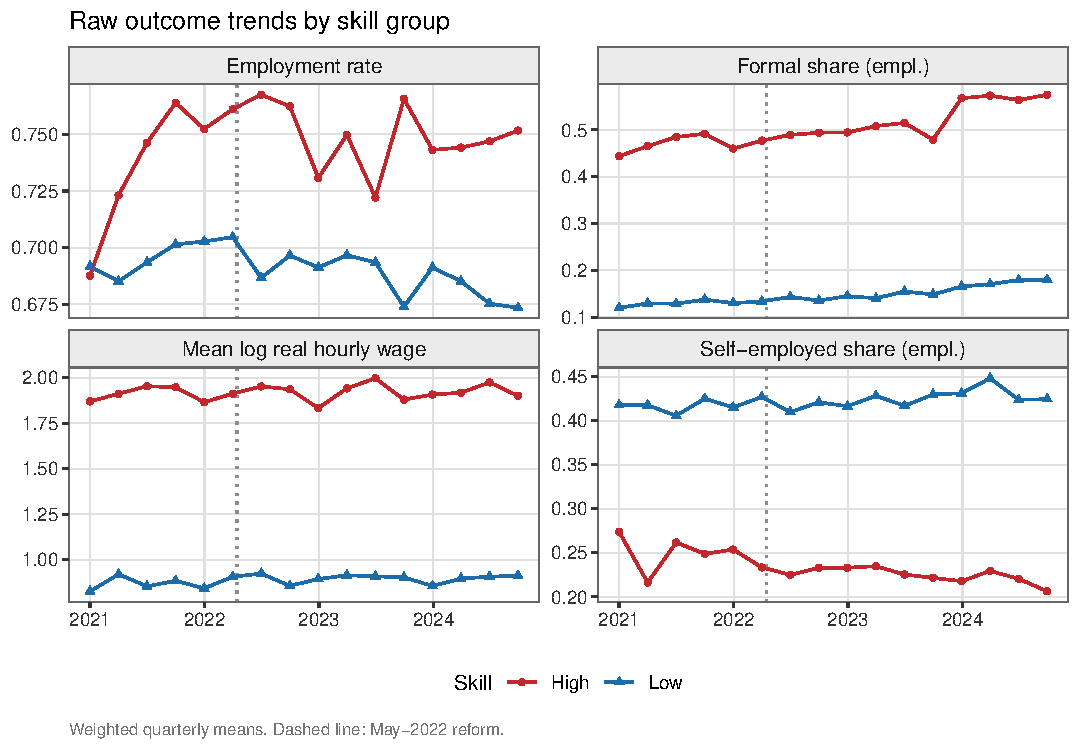
\includegraphics[width=0.95\textwidth]{fig2_raw_trends.pdf}
\caption{Raw outcome trends by skill group, 2021--2024. Weighted quarterly means for
low- and high-skilled workers. The dashed vertical line marks the May 2022 reform.}
\label{fig:trends}
\end{figure}

Figure~\ref{fig:bite} displays the regional variation in the bite of the minimum wage,
measured by the Kaitz index, the ratio of the new minimum to the pre-reform median
dependent wage in each department. The index ranges from about 0.79 in the richest
department to about 2.79 in the poorest, so that in much of the country the new minimum
exceeds the median wage. This variation is predetermined with respect to the reform and
provides the basis for the triple-difference and continuous-intensity checks in
Section~\ref{sec:robustness}.

\begin{figure}[H]
\centering
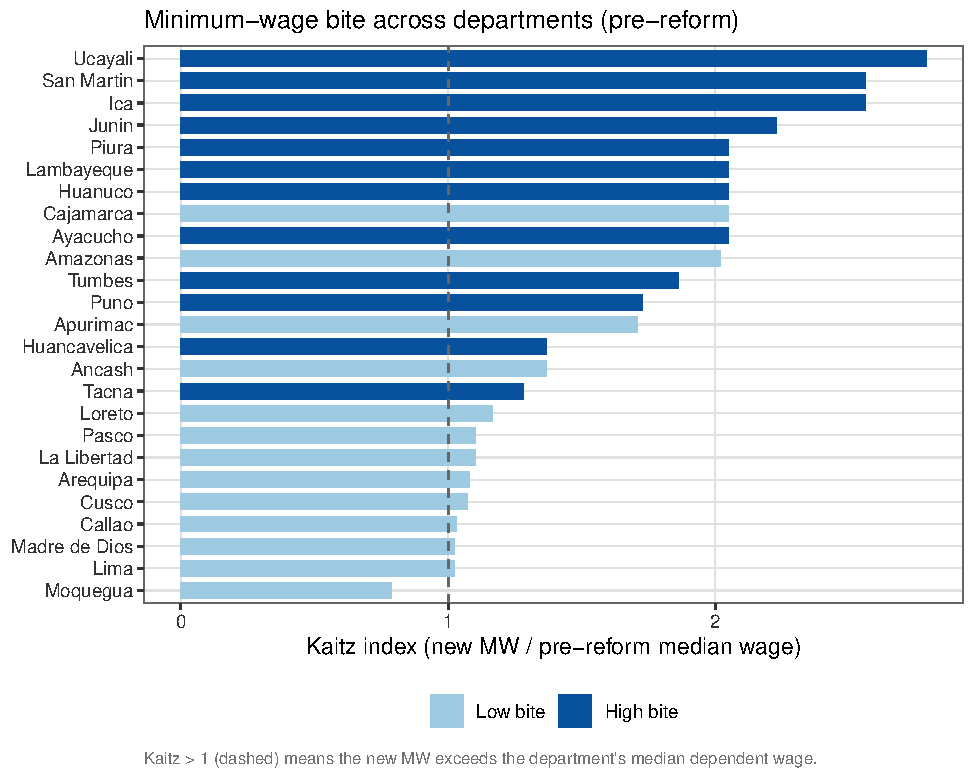
\includegraphics[width=0.72\textwidth]{fig3_regional_bite.pdf}
\caption{Regional variation in the bite of the minimum wage. The Kaitz index is the
ratio of the new minimum wage (1,025 soles) to the department's median monthly wage of
dependent employees in the pre-reform quarters. Departments above the dashed line have
a median wage below the new minimum.}
\label{fig:bite}
\end{figure}

\section{Empirical strategy}\label{sec:strategy}

\subsection{Potential outcomes and the estimand}

Let $i$ index individuals, $g\in\{\Low,\mathrm{High}\}$ their skill group, and $t$ the
quarter. The reform becomes effective in the second quarter of 2022, which I denote
$t^{\ast}$; define the post-reform indicator $\Post_t=\mathbf{1}\{t\ge t^{\ast}\}$ and
the treatment indicator $\Low_i=\mathbf{1}\{g_i=\Low\}$. Following the potential-outcomes
framework, let $Y_{it}(1)$ and $Y_{it}(0)$ denote the outcome of individual $i$ in
quarter $t$ with and without the reform being in force. The parameter of interest is the
average effect of the reform on the low-skilled, relative to the counterfactual in which
they had experienced the same evolution as the high-skilled,
\begin{equation}
\mathrm{ATT} \;=\; \mathbb{E}\!\left[\,Y_{it}(1)-Y_{it}(0)\;\middle|\;\Low_i=1,\;t\ge t^{\ast}\right].
\end{equation}
The data are repeated cross-sections rather than a panel, so the object is identified from
comparisons of group means over time rather than from within-person changes.

Because Peru's minimum wage is national and changes on a single date, there is no variation
in treatment \emph{timing}; every worker is exposed to the same policy at the same moment.
Identification instead rests on variation in the \emph{intensity} of exposure across skill
groups. The design is therefore a canonical two-group difference-in-differences with many
periods, not a staggered-adoption design. This distinction matters for the choice of
estimator. The recent econometric literature has shown that the two-way fixed-effects
estimator can be badly biased when treatment timing is staggered and effects are
heterogeneous \citep{goodmanbacon_2021, dechaisemartin_2020, sun_abraham_2021,
callaway_santanna_2021}. With a common treatment date, however, these problems do not
arise: the two-way fixed-effects estimator and its event-study analog recover a convex,
properly weighted average of treatment effects \citep{roth_2023_trending,
baker_larcker_wang_2022}. I nonetheless report the doubly robust estimator of
\citet{santanna_zhao_2020} as a complementary building block.

\subsection{Estimating equations}

My baseline specification is the two-way fixed-effects difference-in-differences model
\begin{equation}
Y_{idt} \;=\; \beta\,(\Low_i\times\Post_t) \;+\; \gamma\,\Low_i \;+\; \lambda_t \;+\; \mu_d
\;+\; X_{it}'\theta \;+\; \varepsilon_{idt},
\label{eq:twfe}
\end{equation}
where $d$ denotes the department, $\lambda_t$ are quarter fixed effects, $\mu_d$ are
department fixed effects, and $X_{it}$ is a vector of controls comprising age, its square,
sex, an urban indicator, marital status, and years of education (which captures variation
in attainment within skill groups). The coefficient $\beta$ is the difference-in-differences
estimate. The quarter fixed effects absorb any shock common to both skill groups in a given
quarter, including aggregate inflation, so that estimates in logs are invariant to whether
wages are expressed in nominal or in nationally deflated real terms. Observations are
weighted by the survey weights, and standard errors are clustered by department.

To trace the dynamics of the effect and to test the identifying assumption, I estimate the
dynamic event-study specification
\begin{equation}
Y_{idt} \;=\; \sum_{k\neq -1}\beta_k\,\bigl(\Low_i\times\mathbf{1}\{t-t^{\ast}=k\}\bigr)
\;+\; \gamma\,\Low_i \;+\; \lambda_t \;+\; \mu_d \;+\; X_{it}'\theta \;+\; \varepsilon_{idt},
\label{eq:event}
\end{equation}
where $k$ indexes quarters relative to the reform and the quarter immediately before the
reform ($k=-1$, the first quarter of 2022) is the omitted reference. The coefficients
$\beta_k$ for $k<0$ measure differential pre-trends between the skill groups and provide a
direct test of parallel trends; the coefficients for $k\ge 0$ trace the path of the effect.

\subsection{Identifying assumptions and threats}

Identification of the ATT from equation~\eqref{eq:twfe} requires that, absent the reform, the
outcomes of low- and high-skilled workers would have followed parallel paths, conditional on
the controls and fixed effects. Three threats deserve attention.

First, \emph{differential trends}. Education is correlated with sector, region, and formality,
and the two skill groups could have been on diverging paths for reasons unrelated to the
minimum wage. I assess this directly through the pre-reform event-study coefficients and a
joint test of their equality to zero, and I probe robustness to department-specific linear
trends. Because my window opens in the depth of the pandemic recovery, when the employment of
low- and high-skilled workers rebounded at different rates, I pay particular attention to the
first quarter of 2021 and report specifications that drop it.

Second, \emph{sensitivity to residual violations}. Even when pre-trends are statistically flat,
they need not be exactly zero. I therefore report the sensitivity analysis of
\citet{rambachan_roth_2023}, which asks how large a post-reform violation of parallel trends,
relative to the largest violation observed before the reform, would be needed to overturn each
conclusion.

Third, \emph{spillovers and general equilibrium}. If the reform displaces low-skilled workers
into the informal sector, it may indirectly depress wages there, and if high-skilled workers are
imperfect substitutes their outcomes could also move, contaminating the comparison group. I
cannot rule this out, and I interpret the estimates as relative effects. The comparison group is not
entirely unexposed, since a minority of high-skilled workers also earn near the floor through
informal or own-account work; this imperfect exposure attenuates my estimates toward zero, so
the design understates rather than overstates the true effect on the fully exposed. I assess the
plausibility of the comparison by showing that the median high-skilled wage sits well above the
floor and that the high-skilled event-study path shows no break at the reform.

\subsection{Inference}

The treatment is assigned at a coarse level, the skill group, which raises the standard concern
that conventional standard errors overstate precision \citep{bertrand_2004}. I address this in
several complementary ways. My baseline clusters by department, which allows arbitrary
within-department correlation across individuals and quarters; I report an alternative that
clusters by department and skill group; and I apply the bias-reduced CR2 small-sample correction
of \citet{pustejovsky_tipton_2018} to department-level collapsed cells, where it is
computationally feasible. Because these corrections may still be optimistic with a two-group
design, I complement them with randomization inference at the department level, permuting the
regional bite of the minimum wage across departments to construct an exact null distribution for
the exposure-intensity design.

\section{Main results}\label{sec:results}

\subsection{The wage response}

The central result of the paper is that the 2022 reform did not raise the real wages of
low-skilled workers relative to high-skilled workers. Column (1) of
Table~\ref{tab:main} reports the two-way fixed-effects difference-in-differences
estimate from equation~\eqref{eq:twfe}. The coefficient on the interaction of the
low-skill indicator with the post-reform indicator is $-0.009$ for the log real hourly
wage, with a standard error of $0.022$, an estimate that is economically small and
statistically indistinguishable from zero. The implied point estimate is a relative
change of less than one percent, and the ninety-five percent confidence interval rules
out relative wage gains larger than about three percent. The result for log monthly
earnings is likewise a tight null. The doubly robust estimator of
\citet{santanna_zhao_2020} in column (2) is negative and imprecise but tells the same
qualitative story of no positive wage effect.\footnote{The doubly robust estimator collapses
the data to a single pre- and post-reform period and omits department fixed effects, so it is
less comparable to the two-way fixed-effects specification and the event study; I report it as
a complementary check rather than as the preferred estimate.}

The dynamic event study confirms that this null is not an artifact of averaging over
offsetting periods. The top-left panel of Figure~\ref{fig:event} plots the coefficients
$\beta_k$ from equation~\eqref{eq:event} for the log real hourly wage. The pre-reform
coefficients are small and statistically insignificant, and a joint test of their
equality to zero does not reject, with a $p$-value of $0.60$ reported in column (3) of
Table~\ref{tab:main}. After the reform the coefficients hover around zero with no
discernible break. The wage distribution tells a consistent story:
Figure~\ref{fig:dist} shows the earnings distribution of low-skilled wage employees
before and after the reform, with the old and new minima marked. There is a visible mass
of workers near the old minimum, but the distribution does not shift appreciably toward
the new floor, and a large share of workers remain below it, reflecting the pervasive
non-compliance documented in Section~\ref{sec:data}.

\begin{table}[!tbp]\centering
\caption{Difference-in-differences estimates of the 2022 minimum-wage reform}\label{tab:main}
\begin{threeparttable}
\footnotesize
\setlength{\tabcolsep}{4pt}
\begin{tabular}{lcccc}
\toprule
Outcome & (1) TWFE DiD & (2) Doubly robust & (3) Pre-trend $p$ & (4) Elasticity \\
\midrule
Log real hourly wage & -0.021 & -0.056 & 0.001 & -0.20 \\
 & (0.012) & (0.137) & & \\
 & \multicolumn{2}{c}{\footnotesize $N=69,534$, $\bar{y}=1.744$} & & \\
Log real monthly earnings & -0.010 & -0.047 & 0.079 & -0.10 \\
 & (0.013) & (0.097) & & \\
 & \multicolumn{2}{c}{\footnotesize $N=70,691$, $\bar{y}=6.901$} & & \\
Employment & -0.025$^{***}$ & 0.020 & 0.000 & -0.35 \\
 & (0.006) & (0.037) & & \\
 & \multicolumn{2}{c}{\footnotesize $N=278,064$, $\bar{y}=0.707$} & & \\
Labour force participation & -0.008$^{*}$ & -0.015 & -- & -0.10 \\
 & (0.004) & (0.034) & & \\
 & \multicolumn{2}{c}{\footnotesize $N=278,064$, $\bar{y}=0.744$} & & \\
Formal employment & -0.046$^{***}$ & 0.006 & 0.148 & -1.99 \\
 & (0.007) & (0.040) & & \\
 & \multicolumn{2}{c}{\footnotesize $N=181,317$, $\bar{y}=0.228$} & & \\
Self-employment & 0.036$^{***}$ & 0.046 & 0.003 & 0.91 \\
 & (0.006) & (0.045) & & \\
 & \multicolumn{2}{c}{\footnotesize $N=181,317$, $\bar{y}=0.389$} & & \\
Weekly hours & 0.556$^{**}$ & -0.424 & 0.034 & 0.13 \\
 & (0.249) & (0.872) & & \\
 & \multicolumn{2}{c}{\footnotesize $N=179,111$, $\bar{y}=40.655$} & & \\
Paid below the MW & -0.006 & -0.007 & 0.128 & -0.16 \\
 & (0.007) & (0.039) & & \\
 & \multicolumn{2}{c}{\footnotesize $N=70,691$, $\bar{y}=0.352$} & & \\
\bottomrule
\end{tabular}
\begin{tablenotes}\footnotesize
\item Notes: Each row is a separate regression on ENAHO 2021Q1--2024Q4, excluding the partially treated transition quarter 2022Q2. Column (1) reports the two-way fixed-effects DiD coefficient on $\mathrm{Low}\times\mathrm{Post}$ from equation~\eqref{eq:twfe}, with department and quarter fixed effects and controls (age, age squared, sex, urban, marital status, years of education). Column (2) reports the doubly robust DiD estimator of \citet{santanna_zhao_2020} collapsing to pre/post; its standard errors are clustered by department using the estimator's influence function. Column (3) is the $p$-value of a joint test that the pre-reform event-study interactions are zero. Column (4) converts the column-(1) estimate into an elasticity with respect to the 10.2 percent minimum-wage increase (for level outcomes, relative to the baseline mean $\bar{y}$). Wage outcomes are for private-sector wage earners (employees and domestic workers, monthly-equivalent earnings); formality, hours, and self-employment are for private-sector workers. Standard errors clustered by department (25 clusters) in parentheses; all estimates are weighted by ENAHO survey weights. $^{*}p<0.1$, $^{**}p<0.05$, $^{***}p<0.01$.
\end{tablenotes}
\end{threeparttable}\end{table}


That the reform failed to lift wages at the bottom is not surprising in this setting: once
inflation is netted out the real value of the floor rose little, and most low-skilled workers
are informal or self-employed, so the statutory minimum binds for only a minority of them. The
precise null also contrasts with the ``lighthouse'' pattern that \citet{jimenez_2023} finds
for the 2016 reform. I take up these mechanisms, and the contrast with earlier reforms, in
Section~\ref{sec:discussion}.

\subsection{Employment and its composition}

If the reform did not raise pay, did it affect employment or its composition? Here the
evidence is more suggestive than conclusive, and it points to adjustment along the margin
between formal and informal work rather than to large changes in the level of employment.

The estimated effect on the probability of formal employment among the employed is
$-0.036$ (column 1 of Table~\ref{tab:main}), a decline of about three and a half
percentage points for low-skilled relative to high-skilled workers, and it is precisely
estimated under department clustering. The pre-trend test does not reject parallel trends
($p=0.44$), and the event study in Figure~\ref{fig:event} shows relative formality of the
low-skilled drifting down after the reform. Mirroring this, the probability of
self-employment rises by about three percentage points, an estimate that is statistically
significant and, as shown below, robust to randomization inference. Taken together these
two results describe a reallocation of low-skilled workers away from formal salaried jobs
and toward own-account work, the classic informalization margin emphasized by
\citet{jaramillo_lopez_2006} for Peru and by \citet{ham_2018_honduras} for Honduras. Weekly hours
in the main occupation rise modestly, consistent with a shift toward self-employment,
where hours are less constrained.

The effect on the overall employment rate is negative, at about $-2.5$ percentage points,
but it is the least robust of my estimates. As the event study makes clear, the employment
series carries a differential pre-trend concentrated in the first quarter of 2021, when the
labor market was still recovering unevenly from the pandemic across skill groups. Once that
quarter is excluded the pre-trend test no longer rejects, but the point estimate also
attenuates, and the effect does not survive my more conservative inference procedures. I
therefore treat the employment-level result as inconclusive and place little weight on it,
reserving the interpretive emphasis for the compositional shift, which is more stable.
Finally, the indicator for being paid below the minimum shows no significant change, meaning
that the reform did not measurably improve compliance at the bottom of the distribution.

\begin{figure}[H]
\centering
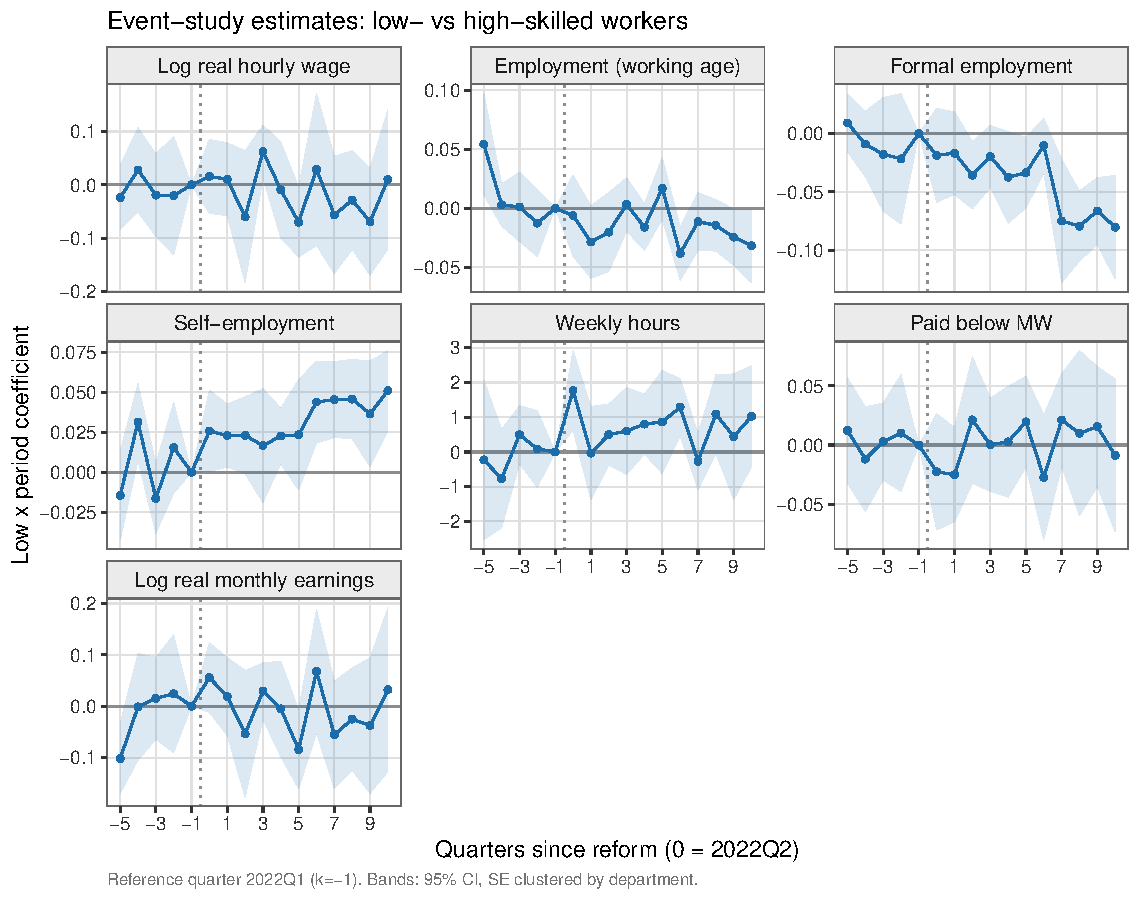
\includegraphics[width=0.98\textwidth]{fig5_event_study.pdf}
\caption{Event-study estimates of the 2022 reform. Each panel plots the coefficients
$\beta_k$ on the interaction of the low-skill indicator with quarter indicators from
equation~\eqref{eq:event}, relative to the omitted quarter 2022Q1 ($k=-1$). The reform is
effective at $k=0$ (2022Q2). Shaded bands are ninety-five percent confidence intervals with
standard errors clustered by department.}
\label{fig:event}
\end{figure}

\begin{figure}[H]
\centering
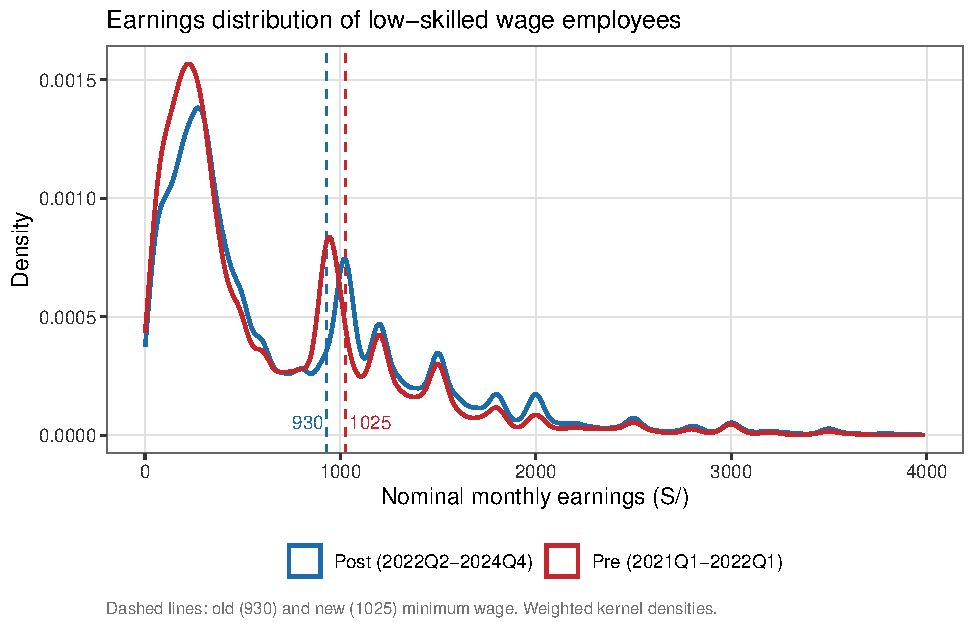
\includegraphics[width=0.72\textwidth]{fig4_wage_distribution.pdf}
\caption{Earnings distribution of low-skilled wage employees, before and after the reform.
Weighted kernel densities of nominal monthly earnings, with the old (930) and new (1,025)
minimum wage marked by dashed lines.}
\label{fig:dist}
\end{figure}

\section{Robustness and inference}\label{sec:robustness}

This section subjects the main results to a battery of specification, inference, and
design checks, and then to an out-of-sample replication. The overall message is that the
compositional results, the decline in formality and the rise in
self-employment, are the most robust findings, corroborated by an independent
continuous-exposure design under randomization inference; the wage evidence consistently
shows no pay gain but carries a pre-trend caveat; and the employment-level result fails
its diagnostics and should not be read causally.

\subsection{Specification robustness}

Table~\ref{tab:robspec} reports the $\mathrm{Low}\times\mathrm{Post}$ coefficient for the
four headline outcomes under ten alternative specifications: dropping the controls,
dropping the pandemic quarter of early 2021, adding department-specific linear trends,
restricting to prime-age workers, using an alternative education cutoff that removes the
categories at the boundary between the two groups, adding occupation and industry fixed
effects, clustering by department and skill, restoring the partially treated transition
quarter 2022Q2, excluding agriculture (which is covered by the separate agrarian labor
regime of Ley 31110 rather than the general minimum wage), and adding public-sector
workers back into the job-conditional samples. The formality and self-employment
estimates are stable in sign and magnitude throughout, moving within a narrow band. The
wage estimate is negative or null in every specification and never significantly
positive. The employment estimate, by contrast, attenuates noticeably when the pandemic
quarter is dropped or when department-specific trends are included, which reinforces my
reluctance to interpret it causally.

\begin{table}[!tbp]\centering
\caption{Specification robustness of the DiD estimates}\label{tab:robspec}
\begin{threeparttable}
\footnotesize
\begin{tabular}{lcccc}
\toprule
Specification & Log hourly wage & Employment & Formal empl. & Self-employment \\
\midrule
Baseline & -0.021 & -0.025$^{***}$ & -0.046$^{***}$ & 0.036$^{***}$ \\
 & (0.012) & (0.006) & (0.007) & (0.006) \\
 & \footnotesize[69,534] & \footnotesize[278,064] & \footnotesize[181,317] & \footnotesize[181,317] \\
No controls & -0.008 & -0.021$^{***}$ & -0.042$^{***}$ & 0.042$^{***}$ \\
 & (0.012) & (0.006) & (0.007) & (0.006) \\
 & \footnotesize[69,534] & \footnotesize[278,064] & \footnotesize[181,317] & \footnotesize[181,317] \\
Drop 2021Q1 (pandemic) & -0.023$^{*}$ & -0.014$^{***}$ & -0.042$^{***}$ & 0.031$^{***}$ \\
 & (0.012) & (0.005) & (0.008) & (0.005) \\
 & \footnotesize[65,279] & \footnotesize[259,135] & \footnotesize[168,908] & \footnotesize[168,908] \\
Department linear trends & -0.022$^{*}$ & -0.017$^{***}$ & -0.040$^{***}$ & 0.034$^{***}$ \\
 & (0.012) & (0.006) & (0.007) & (0.006) \\
 & \footnotesize[69,534] & \footnotesize[278,064] & \footnotesize[181,317] & \footnotesize[181,317] \\
Prime age (25--55) & -0.030$^{*}$ & -0.023$^{***}$ & -0.042$^{***}$ & 0.029$^{***}$ \\
 & (0.015) & (0.004) & (0.008) & (0.007) \\
 & \footnotesize[46,021] & \footnotesize[161,115] & \footnotesize[119,540] & \footnotesize[119,540] \\
Alternative education cutoff & -0.015 & -0.039$^{***}$ & -0.065$^{***}$ & 0.050$^{***}$ \\
 & (0.012) & (0.007) & (0.006) & (0.007) \\
 & \footnotesize[40,526] & \footnotesize[186,263] & \footnotesize[117,174] & \footnotesize[117,174] \\
Occupation \& industry FE & -0.007 & -0.016$^{***}$ & -0.036$^{***}$ & 0.027$^{***}$ \\
 & (0.011) & (0.003) & (0.006) & (0.005) \\
 & \footnotesize[69,534] & \footnotesize[213,810] & \footnotesize[181,317] & \footnotesize[181,317] \\
Cluster dept.$\times$skill & -0.021 & -0.025 & -0.046$^{***}$ & 0.036$^{***}$ \\
 & (0.013) & (0.020) & (0.007) & (0.007) \\
 & \footnotesize[69,534] & \footnotesize[278,064] & \footnotesize[181,317] & \footnotesize[181,317] \\
Low-skilled group linear trend & -0.021 & -0.005 & -0.004 & 0.006 \\
 & (0.019) & (0.008) & (0.010) & (0.009) \\
 & \footnotesize[69,534] & \footnotesize[278,064] & \footnotesize[181,317] & \footnotesize[181,317] \\
Include transition quarter (2022Q2) & -0.018 & -0.025$^{***}$ & -0.044$^{***}$ & 0.035$^{***}$ \\
 & (0.012) & (0.005) & (0.007) & (0.006) \\
 & \footnotesize[74,310] & \footnotesize[296,954] & \footnotesize[193,762] & \footnotesize[193,762] \\
Exclude agriculture (agrarian regime) & -0.022$^{*}$ & -- & -0.038$^{***}$ & 0.028$^{***}$ \\
 & (0.012) &  & (0.007) & (0.005) \\
 & \footnotesize[53,755] & \footnotesize[--] & \footnotesize[114,212] & \footnotesize[114,212] \\
Include public-sector workers & -0.002 & -- & -0.037$^{***}$ & 0.030$^{***}$ \\
 & (0.010) &  & (0.008) & (0.006) \\
 & \footnotesize[87,033] & \footnotesize[--] & \footnotesize[200,383] & \footnotesize[200,383] \\
\bottomrule
\end{tabular}
\begin{tablenotes}\footnotesize
\item Notes: Each cell is the $\mathrm{Low}\times\mathrm{Post}$ DiD coefficient (standard error clustered by department below; sample size in brackets) for the outcome in the column heading, under the specification in the row; all estimates are weighted by ENAHO survey weights, and Log hourly wage denotes the log real hourly wage. The baseline is equation~\eqref{eq:twfe}, which excludes the partially treated 2022Q2. The alternative education cutoff defines low-skilled as at most incomplete secondary and high-skilled as at least complete non-university tertiary, dropping the boundary categories. The agriculture exclusion and the public-sector inclusion apply to job-conditional outcomes only (industry and sector are undefined for non-workers). $^{*}p<0.1$, $^{**}p<0.05$, $^{***}p<0.01$.
\end{tablenotes}
\end{threeparttable}\end{table}


\subsection{Inference}

Because the treatment contrast varies only across two education groups, conventional
department clustering does not by itself deliver design-based inference for the
$\mathrm{Low}\times\mathrm{Post}$ coefficient, and I therefore report a menu of
progressively more demanding procedures. Table~\ref{tab:inference} collects the
evidence. Columns (1) through (3) report $p$-values for the baseline effect under
department clustering (25 clusters), department-by-skill clustering (50 clusters), and
the CR2 small-sample correction of \citet{pustejovsky_tipton_2018} applied to
collapsed cells in the spirit of \citet{bertrand_2004}, here at the
department$\times$group$\times$period level, which is the finest aggregation at which
the CR2 correction is computationally feasible.
The formality and self-employment effects remain highly significant under both
clustering schemes; under the collapsed-cell CR2 procedure, which is deliberately
conservative and low-powered with twenty-five departments, self-employment remains
marginally significant and formality does not. The employment effect loses significance
under everything beyond simple department clustering. Because a permutation test of the
two-group contrast is undefined, design-based randomization inference is conducted for
the continuous-exposure design instead, where the assignment being permuted (the
regional bite) has twenty-five values: column (4) reports these $p$-values, which
belong to the column-(5) estimates, not to the education contrast.\footnote{A wild
cluster bootstrap in the spirit of \citet{cameron_2008_bootstrap} is not available
for survey-weighted estimation, so the CR2 and randomization procedures play that
role here.}

\begin{table}[!tbp]\centering
\caption{Inference robustness, design robustness, and out-of-sample validation}\label{tab:inference}
\begin{threeparttable}
\footnotesize
\setlength{\tabcolsep}{3.5pt}
\begin{tabular}{lcccccc}
\toprule
Outcome & (1) Dept. & (2) Dept.$\times$sk. & (3) CR2 & (4) RI (cont.) & (5) Continuous & (6) 2025 \\
\midrule
Log hourly wage & 0.106 & 0.126 & 0.854 & 0.029 & 0.017 & 0.002 \\
 & & & & & (0.012) & (0.011) \\
Employment & 0.000 & 0.210 & 0.507 & 0.003 & -0.034$^{***}$ & -0.002 \\
 & & & & & (0.012) & (0.005) \\
Formal empl. & 0.000 & 0.000 & 0.244 & 0.000 & -0.018$^{***}$ & -0.001 \\
 & & & & & (0.003) & (0.008) \\
Self-employment & 0.000 & 0.000 & 0.093 & 0.024 & 0.010$^{**}$ & -0.014$^{**}$ \\
 & & & & & (0.004) & (0.006) \\
\bottomrule
\end{tabular}
\begin{tablenotes}\footnotesize
\item Notes: Columns (1)--(3) report $p$-values for the baseline $\mathrm{Low}\times\mathrm{Post}$ effect under, respectively, department clustering (25 clusters), department$\times$skill clustering (50 clusters), and the CR2 small-sample correction \citep{pustejovsky_tipton_2018} applied to department-level collapsed cells. Column (4) reports the randomization-inference $p$-value for the CONTINUOUS-exposure design of column (5), not for the two-group $\mathrm{Low}\times\mathrm{Post}$ contrast, obtained by permuting the 25 regional Kaitz indices across departments (2{,}000 draws). Column (5) reports the continuous-exposure estimate, the coefficient on $\mathrm{Post}\times$(standardized department Kaitz index), with department-clustered standard errors in parentheses. Column (6) reports the $\mathrm{Low}\times\mathrm{Post}$ DiD estimate for the January-2025 reform (window 2024--2025), with department-clustered standard errors in parentheses. Log hourly wage denotes the log real hourly wage; all estimates are weighted by ENAHO survey weights. $^{*}p<0.1$, $^{**}p<0.05$, $^{***}p<0.01$.
\end{tablenotes}
\end{threeparttable}\end{table}


\subsection{Design robustness: bite intensity and triple differences}

My identification rests on differential exposure by education, but the minimum wage also
bites differentially across regions, and this provides an independent source of
variation that does not rely on the education contrast at all. Column (5) of
Table~\ref{tab:inference} reports a continuous-exposure specification in the spirit of
\citet{card_1992}, which relates outcomes to the standardized pre-reform department
Kaitz index interacted with the post indicator. The results corroborate the skill-based
design on the compositional margins: in departments where the minimum wage bites harder,
formal employment falls by 1.8 percentage points more per standard deviation of exposure
($p<0.001$; randomization $p<0.001$) and self-employment rises by 1.0 point more
($p=0.02$; randomization $p=0.02$) after the reform. Employment also declines with
exposure in this design, though I discount that margin for the reasons above. Wages show
no significant response. A triple-difference specification that interacts the skill
contrast with an indicator for high-bite departments is not statistically significant
for any outcome (Appendix Table~\ref{tab:ddd}), which I read as a lack of power in the
coarse binary regional split rather than as evidence against the mechanism, given that
the continuous version is informative and that the subgroup estimates in
Section~\ref{sec:heterogeneity} move in the expected direction.

Three further design checks qualify this corroboration (Appendix
Tables~\ref{tab:expocells} and~\ref{tab:sectorocc}). First, the regional design passes
its own leads diagnostic exactly where it matters: joint tests of the pre-reform
quarter$\times$exposure interactions do not reject for formality ($p=0.84$),
self-employment ($p=0.20$), or wages ($p=0.24$), and reject only for employment
($p=0.002$), consistent with everything else about that margin. Second, in the spirit
of full transparency I also estimate finer, cell-level fraction-affected designs
\citep{card_1992, clemens_wither_2019}, with exposure measured within
department$\times$skill$\times$age cells; these fail their leads diagnostics in both
variants: fine-grained exposure is confounded with the cells' heterogeneous pandemic
recoveries, and the between-floors variant even flips signs because cells with mass
between the two floors are precisely the semi-formal cells that recovered fastest. I
therefore treat the department as the credible level for exposure variation and
report the cell designs in the appendix rather than suppressing them. Third, the
reallocation is broad-based across sectors: the formality decline appears in the
covered high-bite sectors, in other private sectors, and in agriculture alike. The
agricultural estimate is not a falsification failure, because the agrarian regime's
daily remuneration is indexed to the RMV and therefore rose with the reform;
Peru leaves no large sector's floor unchanged, which is why coverage contrasts cannot
be sharp here. An occupation-level dose response (exposure measured as the pre-reform
share of the occupation's wage earners below the new floor) shows larger declines in
sub-floor pay and, suggestively, relative wage gains in more-exposed occupations,
though occupation is measured post-treatment and I read that panel as descriptive.

As a final design check I estimate synthetic difference-in-differences
\citep{arkhangelsky_2021_sdid} on department-by-quarter cells, treating high-bite
departments as treated from 2022Q3 and letting the estimator re-weight low-bite
departments to reconstruct their pre-reform path (Appendix
Table~\ref{tab:sdidpower}). The estimates are directionally consistent with the
reallocation (formality falls and self-employment rises, whether the outcome is the
low-education mean or the low-minus-high skill gap), with magnitudes about half the
TWFE estimates and precision limited by twenty-five aggregate units; the formality
decline in low-education means is significant at five percent under the jackknife.

\subsection{Selection and power}

Because the reform moved workers out of the wage-earner sample, the wage DiD
conditions on an endogenous population. Appendix Table~\ref{tab:leemde} bounds the
resulting bias with the trimming approach of \citet{lee_2009}: the reform reduced
low-skilled wage-sample inclusion by 2.1 percentage points (7.6 percent of the
baseline rate), and trimming the low$\times$post wage distribution by that fraction
from either tail brackets the unconditional 2$\times$2 wage DiD between $-0.10$ and
$+0.10$. Selection alone could therefore mask wage effects of up to ten log points in
either direction, a candid statement of what the wage evidence can and cannot rule
out; the compliance and bunching evidence of Section~\ref{sec:results}, which
conditions only on formality status, is not subject to this concern and is where I
rest the enforcement conclusion. The same appendix table reports minimum detectable
effects: at eighty percent power the design can detect wage effects of 3.4 log
points, and effects of 2.1 and 1.7 percentage points on formality and
self-employment, both well below the estimated 4.6 and 3.6, so the compositional
findings are not an artifact of low statistical power.

\subsection{Sensitivity to violations of parallel trends}

Even flat pre-trends are estimated with error, so I apply the sensitivity analysis of
\citet{rambachan_roth_2023}. Figure~\ref{fig:honest} plots the robust confidence set for
the average post-reform effect on employment and formality as I allow the post-reform
violation of parallel trends to be as large as a multiple $\bar{M}$ of the largest
pre-reform violation. The formality and self-employment effects remain bounded away from
zero under exact parallel trends but include zero once violations as large as
$\bar{M}=0.1$ are allowed, and the employment effect includes zero even at
$\bar{M}=0$. This is the weakest link in the education-based design, and I state it
clearly: the compositional results are robust to conventional and to design-based
inference, but not to modest violations of parallel trends in the education contrast.
Their credibility therefore leans on the two pieces of evidence that do not depend on
that contrast: the regional dose-response gradient and the continuous-exposure design
with randomization inference. The power calculation of \citet{roth_2022_pretest}
quantifies why I do not rely on passed pre-tests alone: a linear violation of
parallel trends that my pre-test would detect only half the time would bias the average
post-period formality effect by 0.042, nine tenths of the estimated effect
(Appendix Table~\ref{tab:sdidpower}, Panel B). Passed pre-tests are reassuring but not
conclusive, and I treat them that way throughout the paper.

Timing granularity does not drive the estimates either. Monthly event studies
(Figure~\ref{fig:monthly}), which time wage outcomes by the income reference month and
employment outcomes by the interview month, show the formality decline appearing
immediately after May 2022 and persisting, with a suggestive dip in the weeks around
the decree's publication on 3 April; and a quarterly event study that bins the right
tail at $k\ge 8$, rather than estimating eleven free lags, leaves the estimates
unchanged.\footnote{The full monthly and binned coefficient series are included in the
replication package.}

\begin{figure}[!t]
\centering
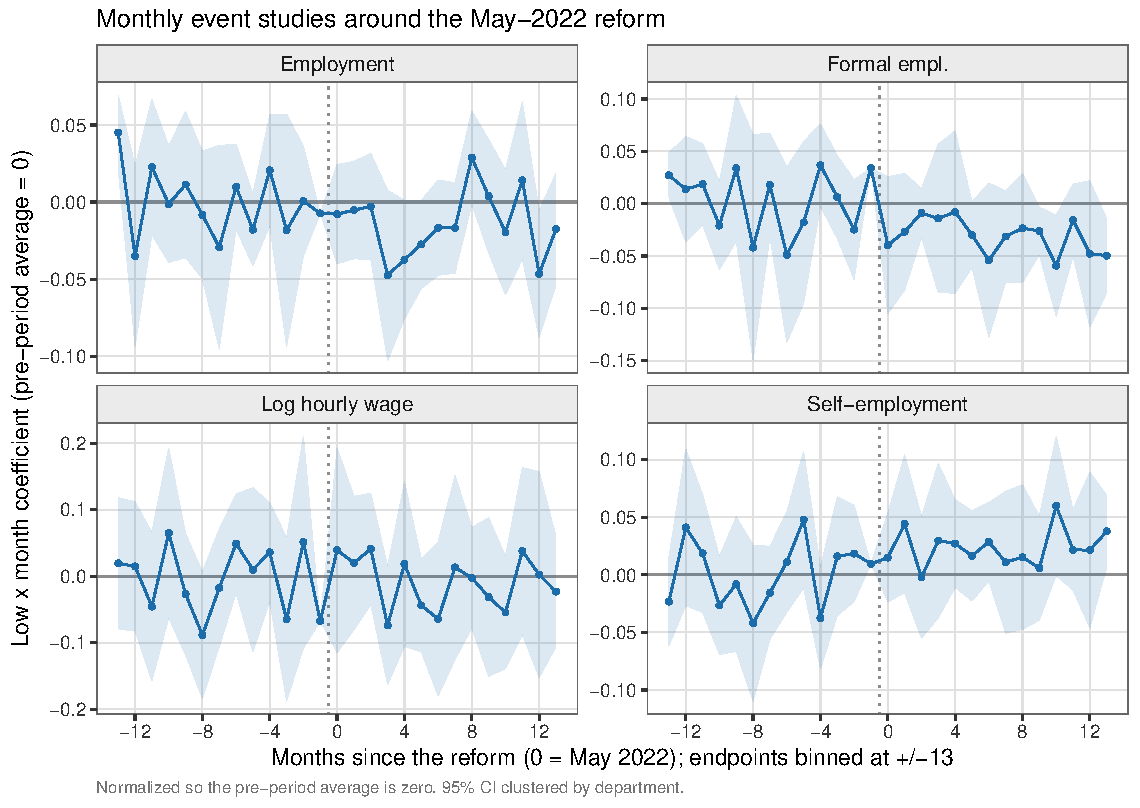
\includegraphics[width=0.98\textwidth]{fig11_monthly_event.pdf}
\caption{Monthly event studies around the May-2022 reform. Wage outcomes are timed by
the income reference month and employment outcomes by the interview month; endpoints
binned at $\pm$13 months; reference month April 2022. Bands: 95 percent confidence
intervals clustered by department.}
\label{fig:monthly}
\end{figure}

\begin{figure}[!t]
\centering
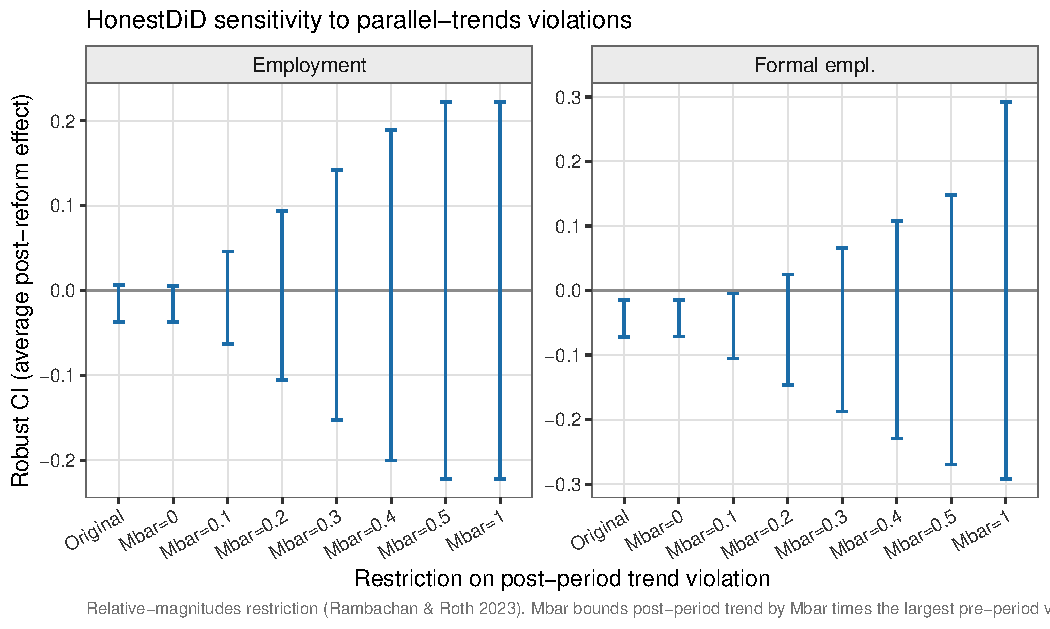
\includegraphics[width=0.8\textwidth]{fig7_honestdid.pdf}
\caption{Sensitivity to violations of parallel trends
\citep{rambachan_roth_2023}. Robust confidence sets for the average post-reform effect
under the relative-magnitudes restriction, which bounds the post-reform trend violation by
$\bar{M}$ times the largest pre-reform violation.}
\label{fig:honest}
\end{figure}

\subsection{Placebo reforms and leave-one-out}

I assign fake reforms to each interior quarter of the pre-reform window and re-estimate
the DiD using only pre-reform data (Appendix Table~\ref{tab:placebo}). The wage placebos
are null and the self-employment placebos are marginal in two of three quarters. The
employment placebos are large and significant in all three quarters, which
is a direct symptom of the pandemic-driven pre-trend in that outcome and the basis for my
refusal to interpret the employment estimate causally.

The formality placebos deserve more than a pass-fail reading, because they and the joint
pre-trend test answer the same question with different power. All three are negative
($-0.024$, $-0.029$, $-0.017$, the last significant at five percent): although the joint
test does not reject ($p=0.15$), the point pattern indicates a downward relative drift of
roughly two percentage points across the pre-window. I therefore quantify how the
formality estimate changes under drift corrections of increasing severity, instead of
relying only on the passed test. Netting out the placebo-implied drift arithmetically leaves
an effect of roughly $-0.02$ to $-0.03$, still more than a tenth of baseline formality
and very close to the synthetic-DiD skill-gap estimate ($-0.028$), which is immune
to group-level drift by construction. Two more aggressive corrections bound the extremes.
A specification that allows the two education groups to diverge along a free linear trend
over the whole window (Table~\ref{tab:robspec}) drives the compositional education-DiD
estimates to zero, but this is mechanical rather than diagnostic: an immediate and persistent
level shift observed over ten post-reform quarters is itself well approximated by a
trend, so this specification absorbs a true step effect along with any drift and is best
read as a worst case. Symmetrically, the smoothness restriction of
\citet{rambachan_roth_2023}, which extrapolates the fitted linear pre-trend into the post
period, yields an uninformative formality interval ($[-0.045,\,0.041]$ at $M=0$):
extrapolating four noisy pre-period points across ten post-period quarters explodes the
variance. The fair summary is that the education contrast alone cannot separate a
persistent level shift from a group trend over a window this long. This is precisely
why the causal weight in this paper rests on the regional-exposure design, whose leads
are flat, whose inference is design-based, and whose dose-response gradient a
group-specific drift cannot generate; and on the convergence of the drift-adjusted
education estimate with the synthetic-DiD estimate at $-0.02$ to $-0.03$.

Leave-one-department-out and leave-one-quarter-out re-estimation
(Appendix Table~\ref{tab:loo}) leaves the point estimates essentially unchanged for all
four outcomes, indicating that no single region or quarter drives the results.

\subsection{A pre-COVID extension of the parallel-trends check}

Because my window opens inside the pandemic recovery, I also test the education
contrast in normal times, using the annual ENAHO employment modules for 2018--2019 and
the quiet window 2018Q3--2019Q4 (after the April-2018 RMV increase and before any
further reform). The exercise is doubly informative. On one hand, it counsels
humility about the education design in levels: joint tests of the
$\mathrm{Low}\times$quarter interactions reject for wages, employment, and
self-employment even in this quiet window: low- and high-education outcomes wobble
relative to each other at low frequencies in normal times, which is an argument for
resting causal weight on the regional-exposure design rather than on the education
contrast alone. On the other hand, the \emph{direction} of the normal-times drift runs
against my 2022 findings, not toward them: a placebo reform placed at 2019Q1 yields a
\emph{negative} self-employment ``effect'' ($-2.2$ percentage points) and a positive,
insignificant formality one ($+0.8$ points), the mirror image of the post-reform
pattern. Whatever secular divergence exists between the groups pushed low-education
workers toward formality and away from self-employment before the pandemic, so it
biases the 2022 reallocation estimates toward zero rather than generating them.

\subsection{Out-of-sample validation: the 2025 reform}

Finally, I replicate the entire design around the second reform, which raised the minimum
wage to 1,130 soles on 1 January 2025, using the 2024 and 2025 quarters. This reform is
of almost identical magnitude to the 2022 one but occurs in a calmer, post-pandemic
environment. Column (6) of Table~\ref{tab:inference} reports the estimates. No wage
response appears ($0.002$, standard error $0.011$): across two reforms in different
macroeconomic conditions, there is no evidence that the minimum wage raised the relative
pay of low-skilled workers. The reallocation, however, does not replicate: the formality
and employment effects are null around the 2025 reform, and the self-employment effect
is small and of the opposite sign. I take this result seriously rather than explain it away. It
implies that the reallocation I document around 2022 is not a stable structural response
that follows every minimum wage increase; it operated in a labor market still
re-sorting after the pandemic, in which marginal formal matches were plausibly easiest
to dissolve. Section~\ref{sec:discussion} develops this state-dependence interpretation
and its alternatives, including the possibility that residual recovery dynamics
contribute to the 2022 estimates.

\section{Heterogeneity and distributional effects}\label{sec:heterogeneity}

\subsection{Who adjusts?}

Figure~\ref{fig:het} reports the low- versus high-skilled DiD estimate for each headline
outcome within demographic and regional subgroups.\footnote{Each estimate is the
within-subgroup difference-in-differences, so it asks whether the low- versus high-skilled
contrast differs across, say, men and women, not the level effect for a subgroup.} Three
patterns stand out and are
consistent with economic intuition about where the minimum wage binds hardest.

First, no subgroup shows wage gains. Whether defined by sex, age, area, or regional bite,
every subgroup wage estimate is negative or indistinguishable from zero. The absence of a
pay response is a pervasive feature of the data rather than an average that masks
offsetting effects.

Second, the compositional adjustment scales with exposure. The decline in formal
employment is larger in high-bite departments ($-5.5$ percentage points) than in low-bite
departments ($-3.6$ points), and the rise in self-employment likewise ($+5.0$ against
$+2.8$ points). This dose-response pattern is what a causal effect of the wage floor
should produce, and it is the cross-sectional counterpart of the continuous-exposure
results in Section~\ref{sec:robustness}. The employment-level estimate, by contrast, does
\emph{not} scale with the bite---it is smaller and insignificant in high-bite
departments---which is further reason to attribute it to differential recovery rather
than to the reform.

Third, the reallocation is concentrated among the young and among women. The decline in
formal employment is largest for workers aged fourteen to twenty-five ($-5.8$ points) and
for women ($-5.5$ points), the groups whose wages are most likely to sit near the floor
and whose attachment to formal employment is most tenuous; the rise in self-employment is
twice as large for women as for men. For workers over forty-five the formality effect is
near zero, though their self-employment also rises. This mirrors the emphasis on youth in
the earlier Peruvian literature \citep{cespedes_2005, jaramillo_lopez_2006} and the
emphasis on women and the least skilled in the developing-country evidence
\citep{katzkowicz_2021_uruguay, lemos_2009}.

\begin{figure}[!t]
\centering
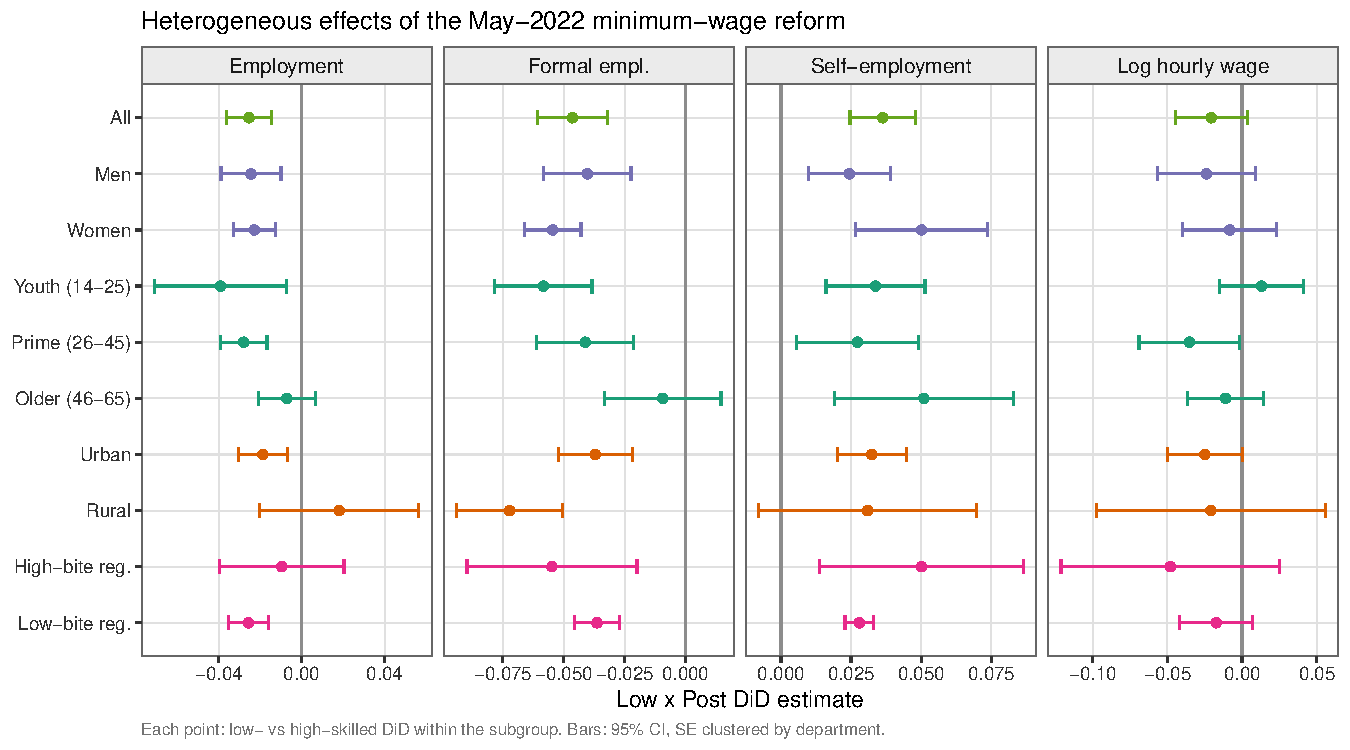
\includegraphics[width=0.98\textwidth]{fig6_heterogeneity.pdf}
\caption{Heterogeneous effects of the 2022 reform. Each point is the
$\mathrm{Low}\times\mathrm{Post}$ DiD estimate within the indicated subgroup, with
ninety-five percent confidence intervals based on standard errors clustered by department.}
\label{fig:het}
\end{figure}

\subsection{Adjustment margins}

Where exactly does the reallocation happen? Four mechanism-oriented margins sharpen
the picture (Appendix Table~\ref{tab:margins}). First, the share of low-education
wage earners employed \emph{without a written contract} rises by 4.5 percentage
points relative to high-education wage earners---informalization operates within
wage employment, not only through exits into self-employment. Second, employment
recomposes toward \emph{micro units}: the probability that a low-education worker is
employed in a establishment of at most twenty workers rises by 2.8 points, and small
units are precisely where enforcement is thinnest. Third, using INEI's decomposition
of informal employment (available through 2023), the displaced margin lands in the
\emph{informal sector} proper (+2.4 points) rather than in unregistered jobs inside
formal firms (+0.8, insignificant): workers did not stay with formal employers under
the table; they moved to informal productive units. Fourth, the share of wage
earners with under a year of tenure does not move, so the adjustment is not visible
as a hiring freeze among those who remain wage earners.

Two further subgroup splits locate the burden. The compositional effects are
concentrated almost entirely among \emph{non-heads} of household---secondary
earners, whose formality falls 6.8 points against a null for household heads---and
among non-indigenous workers, consistent with the urban coastal labor markets where
formal employment at the floor is concentrated. The marginal formal jobs that
dissolved were, in short, those of secondary earners in small urban firms.

\subsection{Distributional wage effects}

The absence of an average wage effect could in principle conceal offsetting movements at
different points of the wage distribution, since a minimum wage is expected to compress the
lower tail. To examine this I estimate unconditional quantile (recentered influence
function) regressions in the manner of \citet{firpo_fortin_lemieux_2009}, applying the DiD
specification to the influence function of each decile of the log real hourly wage.
Figure~\ref{fig:rif} plots the $\mathrm{Low}\times\mathrm{Post}$ coefficient across
deciles. The estimates are non-positive at every decile, mostly between $-2$ and $-4$
percent and significant at a few middle deciles; crucially, there is no positive effect at
the lower deciles, where a binding and enforced minimum wage would compress the
distribution from below. The distributional evidence therefore reinforces the absence of
a pay response: the reform did not lift the lower tail of the low-skilled wage
distribution relative to the high-skilled. This is consistent with the earnings
distribution in Figure~\ref{fig:dist}, which shows little movement toward the new floor,
and with the interpretation that in a labor market with widespread non-compliance the
statutory minimum did not bind for most low-skilled workers.

\begin{figure}[!t]
\centering
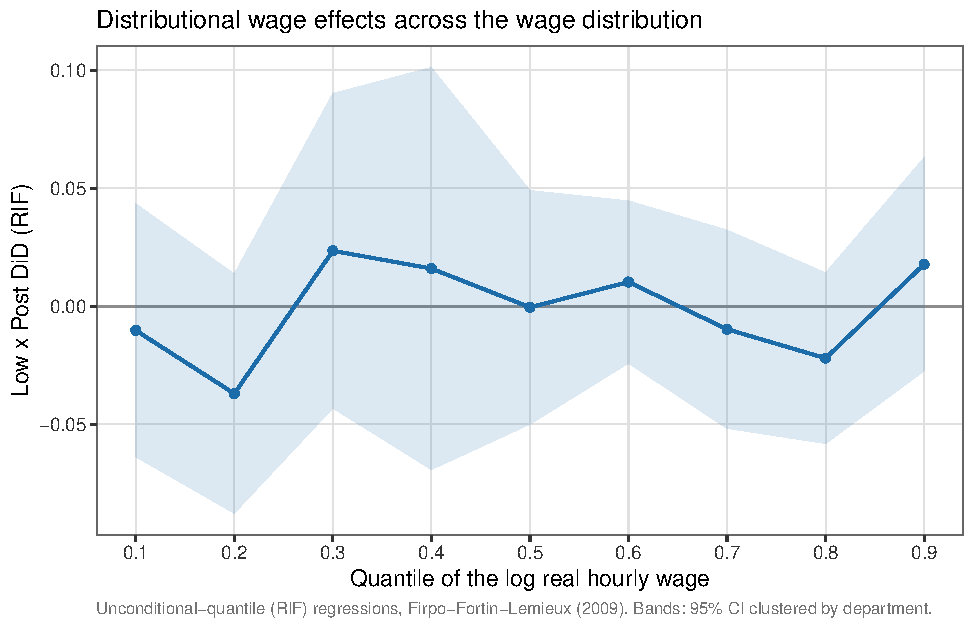
\includegraphics[width=0.72\textwidth]{fig8_rif_quantile.pdf}
\caption{Distributional wage effects. Each point is the $\mathrm{Low}\times\mathrm{Post}$
DiD coefficient from an unconditional-quantile (RIF) regression at the indicated decile of
the log real hourly wage \citep{firpo_fortin_lemieux_2009}. Bands are ninety-five percent
confidence intervals clustered by department.}
\label{fig:rif}
\end{figure}

\section{Discussion}\label{sec:discussion}

\subsection{Mechanisms}

The evidence describes a minimum wage with little purchase on the pay of the workers it is
meant to protect. The wage null is my most robust result: it holds across two reforms, across
the wage distribution, and across demographic groups. Two features of the institutional
environment make it intelligible. The first is inflation. The 2022 increase of ten percent in
nominal terms met consumer price inflation of roughly eight percent, so the real value of the
floor barely rose and then eroded. The second, and more fundamental, is informality. Most
low-skilled Peruvian workers are informal or self-employed, and for them the statutory minimum
is not enforced; compliance is high only within registered formal firms, which employ a
minority of the low-skilled. A floor that reaches only a small and selected part of the
relevant labor force cannot move its average wage by much, and the earnings distribution in
Figure~\ref{fig:dist} confirms that it did not.

If the reform did not raise pay, did it move anything else? Around 2022 I find a shift from
formal employment toward self-employment, concentrated among the young and among women. The
natural mechanism is the classic one, a binding floor in the covered sector inducing some
reallocation to the uncovered sector, the displacement channel that \citet{jaramillo_lopez_2006}
documents for Peru and \citet{ham_2018_honduras} for Honduras; the accompanying rise in hours
is consistent with movement toward self-employment, where hours are less constrained. I read
this cautiously, because the compositional effect does not survive my most demanding inference
and does not reappear around the 2025 reform. Its reversal out of sample suggests that part of
what I capture around 2022 reflects the uneven post-pandemic recovery rather than a structural
response to the minimum wage, so I present the reallocation as a feature of the 2022 episode
rather than as a general law.

\subsection{Reconciliation with the previous literature}

My results sit comfortably with some of the prior evidence and in tension with the rest, and
the pattern is itself informative. They echo the older Peruvian work of
\citet{jaramillo_lopez_2006}, who found the 2003 reform largely innocuous with displacement
toward informality, and of \citet{cespedes_2005}, who found effects concentrated among the
young. They are consistent with the broad international finding that minimum wage increases in
this range produce small employment effects \citep{card_krueger_1995, cengiz_2019}.

The tension is with the most recent Peruvian study. \citet{jimenez_2023} finds that the 2016
reform raised formal wages by four to five percent and increased formality, a lighthouse
pattern that I do not reproduce for 2022. Three differences plausibly account for the
divergence. The 2016 increase occurred in a low-inflation period, so its real bite was larger
and more durable than that of the inflation-eroded 2022 increase. The identification differs:
\citet{jimenez_2023} uses a department-level dose defined on the formal wage distribution,
while I contrast low- and high-education workers at the individual level, a design that places
more weight on the large informal segment of the low-skilled. And the macroeconomic setting
differs, stable growth in 2016 against a post-pandemic recovery in 2022. Taken together, these
suggest that the labor-market effects of the Peruvian minimum wage are state-dependent, closer
to the lighthouse pattern when the real increase is substantial and the economy is stable, and
muted when inflation erodes the increase and informality absorbs the adjustment.

\subsection{External validity and limitations}

Four limitations bound the interpretation. First, identification rests on the assumption that,
absent the reform, low- and high-education workers would have followed parallel paths. I test
this where possible and bound the consequences of its failure, but I cannot rule out
differential shocks correlated with education in the volatile 2021--2022 window; this is why I
lean on the wage result, whose pre-trends are flat and which replicates out of sample, and
treat the employment-level result as inconclusive. Second, the design identifies effects on
low-skilled workers relative to high-skilled workers. If the reform also reached the
high-skilled, through general-equilibrium spillovers or ripple effects up the distribution, my
estimates mismeasure the absolute effect on the low-skilled; I judge large spillovers to the
tertiary-educated unlikely given that their median wage sits well above the floor, and I note
that because the comparison group is not entirely unexposed, any resulting bias attenuates my
estimates toward zero, so the wage null is a conservative reading. Third, the data are repeated
cross-sections, so I cannot follow individuals across the reform or separate changes in the
composition of the employed from changes in individual outcomes. Fourth, informality in 2024
is measured with a reconstructed indicator rather than the official one; my robustness checks
suggest this does not drive the results, but it adds measurement error. Finally, the window
spans at most eleven post-reform quarters, so I speak to short- and medium-run effects and not
to the long-run adjustment of capital or firm entry and exit.

\subsection{Policy implications}

The results carry a sober message for minimum wage policy in a high-informality economy. A
floor that goes unenforced for most of its intended beneficiaries does little to raise their
pay, and where it does bind, in the formal sector, it may nudge some workers toward less
protected arrangements. Raising the minimum wage is therefore an imperfect instrument for
lifting the earnings of the low-skilled in Peru, a conclusion that echoes
\citet{jaramillo_lopez_2006}. This is not to say the minimum wage is harmless or useless; my
estimates are relative and my window is short. But it does imply that formalization and
enforcement are preconditions for the floor to reach the workers it is designed to protect.
Absent them, the margin of adjustment is the composition of employment rather than the level of
pay.

\section{Conclusion}\label{sec:conclusion}

I have studied how Peru's 2022 minimum wage increase, from 930 to 1,025 soles, affected
workers with different levels of education, using quarterly ENAHO data and a
difference-in-differences design that exploits the sharply different exposure of low- and
high-education workers to a single national reform. My central finding is that the reform
shifted the composition of low-skilled employment rather than the level of low-skilled
pay: formal employment fell by 4.6 percentage points, a fifth of its baseline, and
self-employment rose by 3.6 points, with flat formality pre-trends, larger shifts where
the floor cut deeper into the regional wage distribution, and confirmation from a
continuous-exposure design under randomization inference. No pay response accompanied the
shift: relative wages of low-education workers did not rise at the mean or anywhere in
the distribution, and the share of wage earners paid below the floor did not fall,
pointing to non-compliance as the reason the floor could not lift pay. The overall
employment effect cannot be pinned down and is confounded by the uneven post-pandemic
recovery. Around the identically sized reform of January 2025, in a calmer labor market,
neither wages nor composition responded, which suggests that the reallocation margin
operates when the labor market holds many marginal formal matches, as it did during the
post-pandemic re-sorting of 2022, and lies dormant when it does not.

The most economical reading of these results is that, in a labor market where informality
is pervasive and enforcement is weak, a moderate and inflation-eroded increase in the
statutory minimum does not lift the pay of the low-skilled; what it moves, when it moves
anything, is the allocation of workers between formal and informal arrangements. This
qualifies the lighthouse view of the Peruvian minimum wage that emerges from studies of
earlier reforms and points to the informal margin as the central channel of adjustment.

Two directions for future research follow. The first is to exploit panel data, either
the panel component of ENAHO or the higher-frequency EPEN, to follow individuals across
reforms and distinguish worker-level transitions out of formality from changes in the
composition of hiring, which my repeated cross-sections cannot separate. The second is to
study the interaction between minimum wage policy and enforcement directly, since my
results suggest that the returns to raising the floor depend on whether the floor can be
made to bind. As additional post-reform quarters accumulate, it will also become possible
to trace the longer-run adjustment that a short window such as mine cannot capture.


\section*{Declarations}
\noindent\textbf{Declarations of interest:} none.\\
\textbf{Funding:} this research received no specific grant from any funding agency in the
public, commercial, or not-for-profit sectors.\\
\textbf{Data availability:} the ENAHO microdata are publicly available from the Instituto
Nacional de Estad\'istica e Inform\'atica (INEI). The code that reproduces every table and
figure is available in the online replication repository.

\newpage
\bibliography{references}

\newpage
\appendix
\section{Data appendix}\label{app:data}

\subsection{Sample and variable construction}

I pool the twenty quarterly ENAHO employment modules (module 500) for 2021Q1--2025Q4;
the main analysis uses 2021Q1--2024Q4 and the validation uses 2024Q1--2025Q4. The
working-age sample comprises individuals aged 14 to 65 with non-missing education. All
statistics use the module employment weight (\texttt{fac500a}). Departments are the 25
first-level administrative units derived from the first two digits of \texttt{ubigeo};
the urban indicator is derived from the sampling stratum.

\paragraph{Education and skill groups.} Educational attainment is ENAHO variable
\texttt{p301a}. I verified its coding against the weighted attainment distribution.
Low-skilled workers are those with \texttt{p301a} in 1--6 (no education through complete
secondary); high-skilled workers are those with \texttt{p301a} in 7--11 (non-university
higher through postgraduate). Special education (code 12) and missing values are excluded.

\paragraph{Labor income and wages.} For dependent employees, monthly labor income in the
main occupation is the reported gross pay including overtime (\texttt{p524a1}); for
own-account workers it is net profit (\texttt{p530a}). I deflate by the Lima consumer
price index to December 2021 soles. The real hourly wage divides monthly labor income by
$4.345$ times weekly hours in the main occupation (\texttt{p513t}, imputed where missing).
Wages are winsorized at the 0.5th and 99.5th percentiles. As a robustness check I also
construct the imputed, deflated, annualized labor-income aggregate used by
\citet{jimenez_2023}, namely the sum of \texttt{i524a1}, \texttt{d529t}, \texttt{i530a},
and \texttt{d536} divided by twelve; results are unchanged.

\paragraph{Informality.} INEI's official informal-employment indicator (\texttt{ocupinf},
coded 1 for informal and 2 for formal in these files) is present for 2021--2023 but absent
for 2024--2025. I reconstruct a consistent indicator from primitives available in every
year. A wage employee or domestic worker is classified as formal if affiliated to a
pension system (\texttt{p558a1}--\texttt{p558a4}) or holding a formal labor contract
(\texttt{p511a} in 1--6); an employer or own-account worker is classified as formal if the
productive unit is registered (\texttt{p510a1}); unpaid family workers are always informal.
Validated against \texttt{ocupinf} on the overlapping years 2021--2023, this rule agrees
with the official classification for 88.3 percent of employed workers and reproduces the
official informality rate to within about two and a half percentage points. I use the
official indicator wherever available and the reconstruction only for 2024--2025.

\paragraph{Minimum wage and bite.} The statutory minimum wage schedule is taken from the
decrees and verified against the Banco Central de Reserva del Perú series (PN02124PM).
The department Kaitz index is the ratio of the post-reform minimum (1,025 soles) to the
department's pre-reform (2021Q1--2022Q1) weighted median monthly wage of dependent
employees. The fraction-affected measure is the pre-reform weighted share of dependent
employees earning below 1,025 soles.

\subsection{Supplementary results}

Table~\ref{tab:placebo} reports the in-time placebo reforms and confirms that the wage
placebos are null while the employment placebos are contaminated by the pandemic pre-trend.
The doubly robust estimates of \citet{santanna_zhao_2020} appear alongside the two-way
fixed-effects estimates in Table~\ref{tab:main}. Figure~\ref{fig:val2025} shows the
event study around the January-2025 reform used in the out-of-sample validation.

\begin{figure}[H]
\centering
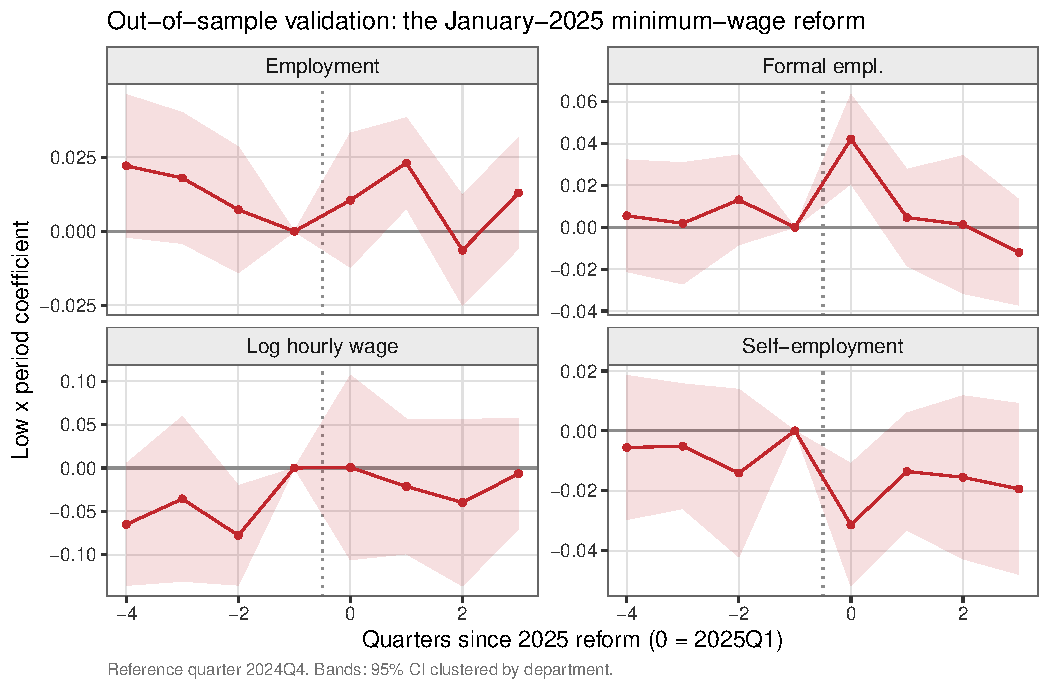
\includegraphics[width=0.9\textwidth]{fig9_validation2025.pdf}
\caption{Event study around the January-2025 reform (out-of-sample validation). Coefficients
on the interaction of the low-skill indicator with quarter indicators, reference quarter
2024Q4. Bands are ninety-five percent confidence intervals clustered by department.}
\label{fig:val2025}
\end{figure}

\begin{table}[H]\centering
\caption{In-time placebo reforms (pre-reform window only)}\label{tab:placebo}
\begin{threeparttable}
\begin{tabular}{lccc}
\toprule
Outcome & Placebo 2021Q2 & Placebo 2021Q3 & Placebo 2021Q4 \\
\midrule
Log real hourly wage & 0.020 & -0.018 & -0.005 \\
 & (0.037) & (0.032) & (0.021) \\
Employment & -0.057$^{***}$ & -0.034$^{***}$ & -0.026$^{***}$ \\
 & (0.016) & (0.007) & (0.008) \\
Formal employment & -0.021$^{*}$ & -0.012 & -0.005 \\
 & (0.011) & (0.013) & (0.007) \\
Self-employment & 0.022$^{*}$ & -0.009 & 0.007 \\
 & (0.012) & (0.007) & (0.009) \\
\bottomrule
\end{tabular}

\begin{tablenotes}\footnotesize
\item Notes: Each entry is the $\mathrm{Low}\times\mathrm{Post}$ coefficient from a placebo
DiD that assigns a fake reform to the indicated quarter, estimated using only pre-reform
data (2021Q1--2022Q1). Standard errors clustered by department in parentheses; all estimates
are weighted by ENAHO survey weights. $^{*}p<0.1$, $^{**}p<0.05$, $^{***}p<0.01$.
\end{tablenotes}
\end{threeparttable}
\end{table}


\end{document}
